% =============================================================
%  Single-phase PLLs: Park PLL, FHT-PLL and DDSRF-PLL of the model single_phase_pll_analysis
%  pwr-control documentation - compile with pdflatex (three times) from inside this folder:
%      pdflatex single_phase_pll.tex  (x3)
%  Block diagrams: TikZ in this file and five Illustrator figures of rev. 00 (figures/*.eps, converted by epstopdf).
%  The figures figures/*.pdf and every number of the note come from the companion script py/make_figures.py
%  (numpy, scipy, matplotlib) with the step-by-step replicas of the three PLL blocks in py/sp_pll_models.py:
%      cd py && python3 make_figures.py [path/to/sim_results_cases.mat]  -> ../figures/*.pdf, single_phase_pll_numbers.txt
%  sim_results_cases.mat is written in the model folder by run_test_cases(1:6, 'sim_results_cases.mat') (not in the
%  repository); without it the script uses the replicas for the test cases too.
% =============================================================
\documentclass[11pt,a4paper]{scrartcl}
% ===================== PACKAGES =====================
\usepackage[british]{babel}
\usepackage[tmargin=1in, bmargin=1in, lmargin=0.75in, rmargin=0.75in]{geometry}
\usepackage[dvipsnames,table]{xcolor}  % prima di tikz, listings, ecc.

\usepackage{tikz}
\usepackage{graphicx}
\usepackage{pgfplots}
\pgfplotsset{width=12cm, compat=1.9}
\usepackage{setspace}
\usepackage{chemmacros}
\usepackage{chemfig}
\usepackage{esint}
\usepackage{tabularray}
\usepackage{makeidx}
\usepackage{epstopdf}
\usepackage{amssymb}
\usepackage{mathrsfs}
\usepackage{bm}
\usepackage{amsmath}
\usepackage{enumitem}
\usepackage[english]{varioref}
\usepackage{lipsum}
\usepackage{fancyhdr}
\usepackage{float}
\usepackage{empheq}
\usepackage[framemethod=tikz]{mdframed}
\numberwithin{equation}{section}
\usepackage{eso-pic}
\usepackage{calc}
\usepackage{nccmath}
\usepackage{caption}
\usepackage{subcaption}
\usepackage{gensymb}
\usepackage{amsfonts, amsthm, epsfig, epstopdf, titling, url, array}
\usepackage{tabularx}
\usepackage{makecell}
\usepackage{booktabs}
\usepackage{array}
\usepackage{siunitx}
\sisetup{input-digits=0123456789\pi}
\usepackage[symbol]{footmisc}
\usepackage{multicol}
\usepackage{boondox-cal}
\usepackage{blindtext}
\usepackage{changepage}
\usepackage{nomencl}
\usepackage{hyperref}
\usepackage{xurl}
\usepackage{ragged2e}
\usepackage[version=4]{mhchem}  % ← conflitto di opzioni
\usepackage{longtable}
\usepackage{chemformula}
\usetikzlibrary{arrows.meta,positioning,calc}

% ===================== SI UNITS =====================
\DeclareSIUnit\atm{atm}
\DeclareSIUnit{\var}{var}
\DeclareSIUnit{\pu}{p.u.}


% ===================== MATH OPERATORS =====================
\DeclareMathOperator{\rank}{rank}
\DeclareMathOperator{\atantwo}{atan2}
\DeclareMathOperator{\spn}{span}

% ===================== COMMANDS =====================
\newcommand{\abs}[1]{\left|#1\right|}
\newcommand{\sign}{\text{sign}}
\newcommand{\centered}[1]{\begin{tabular}{@{}l@{}} #1 \end{tabular}}

% ===================== COLORS =====================
\definecolor{mycolor1}{rgb}{0.97, 0.97, 0.97}
\definecolor{mycolor2}{rgb}{0.97, 0.97, 0.97}
\definecolor{tableShade}{gray}{0.9}

% ===================== THEOREM ENVIRONMENTS =====================
\theoremstyle{it}
\newtheorem{defn}{Definition}[section]
\newtheorem{assumption}{Assumption}[section]
\newtheorem{thm}{Theorem}[section]
\newtheorem{lemma}{Lemma}[section]
\newtheorem{corollary}{Corollary}[section]
\theoremstyle{definition}
\newtheorem{example}{Example}[section]

% ===================== CUSTOM ENVIRONMENTS =====================
\newenvironment{myitemize_1}{
	\begin{itemize}[topsep=0pt]
		\setlength{\topsep}{2pt}
		\setlength{\itemsep}{2pt}
		\setlength{\parskip}{2pt}
		\setlength{\parsep}{2pt}
	}{\end{itemize}}

\newmdenv[
innerlinewidth=0.5pt,
roundcorner=4pt,
backgroundcolor=mycolor2,
linecolor=mycolor1,
innerleftmargin=6pt,
innerrightmargin=6pt,
innertopmargin=6pt,
innerbottommargin=6pt
]{mybox}

% ===================== TABLE COLUMN TYPES =====================
\newcolumntype{Y}{>{\hsize=2\hsize}X}
\newcolumntype{Z}{>{\centering\arraybackslash\hsize=0.857\hsize}X}

% ===================== SECTION DEPTH =====================
\setcounter{secnumdepth}{3}
\setcounter{tocdepth}{3}

% ===================== PAGE STYLE =====================
\setlength{\headheight}{20pt}
\setlength{\headsep}{20pt}

\pagestyle{fancy}
\fancypagestyle{firstpage}{\rhead{}}
\fancyhead[L]{\slshape\nouppercase{\leftmark}}
\chead{}
\rhead{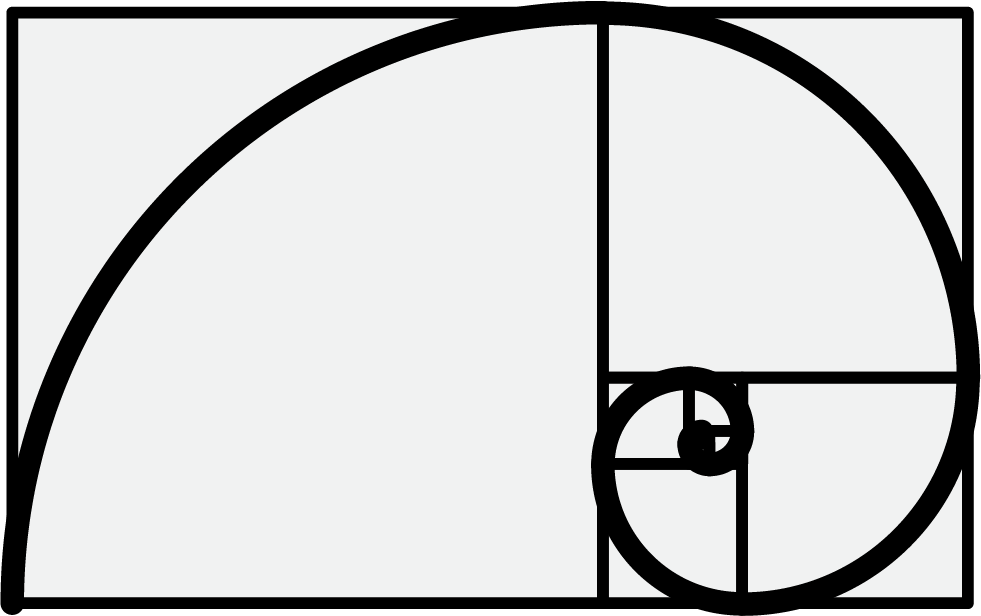
\includegraphics[height=0.75cm]{../../AAA_template_latex_settings/pwr-control_logo_doc.png}}
\lfoot{\href{http://www.pwr-control.com}{pwr-control.com}}
\cfoot{-\ \thepage\ -}
\rfoot{\textit{}}
\renewcommand{\headrulewidth}{0.4pt}
\renewcommand{\footrulewidth}{0.4pt}


\geometry{
	a4paper,
	top    = 2.5cm,
	bottom = 3.0cm,
	left   = 2.5cm,
	right  = 2.5cm
}

\hypersetup{
	colorlinks = true,
	urlcolor   = blue,
	linkcolor  = black,
	citecolor  = black
}

\pagenumbering{gobble}

\usetikzlibrary{shapes.geometric,fit}

\newcommand{\ped}[1]{_{\mathrm{#1}}}
\newcommand{\code}[1]{\texttt{#1}}
\newcommand{\us}{\_\allowbreak}  % breakable underscore for long paths
\newcommand{\sat}{\operatorname{sat}}
\newcommand{\wrapop}{\operatorname{wrap}}
\renewcommand{\tabularxcolumn}[1]{>{\raggedright\arraybackslash}p{#1}}
\setlength{\emergencystretch}{3em}
\sisetup{per-mode=symbol,retain-explicit-plus}

% ---------------- document metadata (read by the title page) ----------------
\newcommand{\DocCategory}{Technical Note}
\newcommand{\DocField}{Power Electronics and Control Systems}

\newcommand{\DocTitle}{%
	{\fontsize{20}{24}\selectfont\bfseries Single-phase phase locked loops\par}
	\vspace{14pt}
	{\fontsize{16}{23}\selectfont\bfseries Park PLL, FHT-PLL and DDSRF-PLL of the model \code{single\_phase\_pll\_analysis}:\\ quadrature signal generators, loop models,\\ test results and what to change\par}
}

\newcommand{\DocSubtitle}{%
	The three phase locked loops that the model \code{single\_phase\_dqPLLs\_analysis} of \code{pwr-control/modelization-and-control} runs side by side on one test voltage, described from the control point of view: the quadrature signal generators and their complex gain, the blocks as they compute, their linear models checked against the simulation, six test cases, the criticalities of each loop and the changes, tested.
}

\newcommand{\DocAuthor}{Davide Bagnara}
\newcommand{\DocRevision}{01}
\newcommand{\DocDate}{November 2026}

\newcommand{\DocAbstract}{%
	The model \code{single\_phase\_pll\_analysis} compares three single-phase phase locked loops on the same test voltage at the control period of \SI{125}{\micro\second}: the Park PLL of the single-phase inverter controls, a PLL fed by first harmonic trackers (FHT-PLL) and a decoupled double synchronous reference frame PLL (DDSRF-PLL), both from the control of the active front end. This revision rewrites the note of 2021 around the model. The quadrature signal generators are compared through one quantity, their complex gain on the components of the input. The Park generator is a SOGI with gain \num{0.5} in disguise, but its phase detector reads the raw input and lets harmonics and DC through with half their amplitude; the first harmonic tracker is a fast and wide observer whose damped, forward Euler model of the oscillator puts its angle \ang{0.74} ahead at \SI{50}{\hertz}. The loops are modelled with the generator inside the loop (Park PLL), outside it (FHT-PLL) and with the exact transfer function of the decoupling network (DDSRF-PLL); the models match the simulation within a few percent up to \SI{100}{\radian\per\second}. On six test cases (sag, phase jump, frequency step, DC offset, harmonics) the Park PLL is the fastest and has no offset, but its loop is of type 1 (\ang{1.15} of error after a \SI{1}{\hertz} step) and its ripple is the largest (\ang{3.4}); the FHT-PLL leads by \ang{1.49} and has \ang{2} to \ang{3} of ripple; the DDSRF-PLL has the lowest ripple (\ang{0.3} to \ang{0.4}) but the slowest response (\SI{89}{\milli\second} after a \ang{30} jump) and a start of up to \SI{180}{\milli\second}. Three changes are proposed and tested on Python replicas that reproduce the model within \num{4e-13} rad: an integral gain for the Park PLL, the undamped tracker with exact discretization (an option of the init) and the start of the DDSRF frequency integrator at \num{1} pu. The SOGI-PLL detector for the Park PLL, DC estimators and narrower trackers are options with a price, given with their numbers.
}

\newcommand{\RevisionHistory}{%
	00 & May 2021 & First issue: basic PLL, SOGI-QSG and Park-based PLL, laboratory implementation on dSPACE SCALEXIO. & \DocAuthor \\
	01 & November 2026 & Rewritten together with the model \code{single\_phase\_dqPLLs\_analysis} (new init): complex gain of the quadrature generators, the three PLLs of the model, linear models checked against the simulation, six test cases, criticalities and changes, scripts \code{py/make\_figures.py} and \code{py/sp\_pll\_models.py}; derivations of rev.~00 corrected, laboratory part removed. & \DocAuthor \\
}

\newcommand{\MetaLabelA}{Project Repository}
\newcommand{\MetaValueAUrl}{https://github.com/pwr-control/modelization-and-control.git}
\newcommand{\MetaValueALabel}{modelization-and-control.git (single\_phase\_dqPLLs\_analysis)}

\newcommand{\MetaLabelB}{Framework}
\newcommand{\MetaValueB}{MATLAB/Simulink, Python}

\begin{document}

% =============================================================
%  pwr-control LaTeX template - FRONTESPIZIO
%
%  Da richiamare come prima istruzione dopo \begin{document}:
%      % =============================================================
%  pwr-control LaTeX template - FRONTESPIZIO
%
%  Da richiamare come prima istruzione dopo \begin{document}:
%      % =============================================================
%  pwr-control LaTeX template - FRONTESPIZIO
%
%  Da richiamare come prima istruzione dopo \begin{document}:
%      \input{../../AAA_template_latex_settings/titlepage}
%
%  Il documento deve definire prima di \begin{document}:
%      \DocCategory   categoria del documento
%      \DocField      area tecnica
%      \DocTitle      titolo (una o due righe)
%      \DocSubtitle   sottotitolo
%      \DocAuthor     autore/i, separati da virgola
%      \DocRevision   numero di revisione corrente (es. 00)
%      \DocDate       data della revisione corrente
%      \DocAbstract   abstract
%      \RevisionHistory  righe della tabella di revisione, nel formato
%                        Rev. & Date & Description & Authors \\
%      \MetaLabelA \MetaValueAUrl \MetaValueALabel
%      \MetaLabelB \MetaValueB
% =============================================================

\providecommand{\DocCategory}{Technical Research Report}
\providecommand{\DocField}{Power Electronics and Control Systems}
\providecommand{\DocSubtitle}{}
\providecommand{\DocRevision}{00}
\providecommand{\DocAbstract}{}
\providecommand{\RevisionHistory}{%
	\DocRevision & \DocDate & First issue. & \DocAuthor \\
}

\titlepage

% ---- Intestazione centrata ----
\begin{center}
	{\Large\scshape \DocCategory}\\[8pt]
	{\large\scshape \DocField}
\end{center}

\vspace{30pt plus 4pt minus 14pt}
\noindent\rule{\linewidth}{0.8pt}

% ---- Titolo ----
\begin{center}
	\DocTitle
\end{center}

\vspace{4pt}
\noindent\rule{\linewidth}{2.2pt}

% ---- Sottotitolo ----
\begin{center}
	\begin{onehalfspace}
		{\large\itshape \DocSubtitle}
	\end{onehalfspace}
\end{center}

% ---- Authors / Revision / Date ----
\vspace{30pt plus 4pt minus 14pt}

\noindent
\begin{minipage}[t]{0.46\linewidth}
	\raggedright
	\textbf{Authors:}\\[2pt]
	\DocAuthor
\end{minipage}%
\hfill
\begin{minipage}[t]{0.22\linewidth}
	\centering
	\textbf{Revision:}\\[2pt]
	\DocRevision
\end{minipage}%
\hfill
\begin{minipage}[t]{0.30\linewidth}
	\raggedleft
	\textbf{Date:}\\[2pt]
	\DocDate
\end{minipage}

\vspace{10pt}
\noindent\rule{\linewidth}{0.8pt}

% ---- Abstract ----
\vspace{24pt plus 4pt minus 12pt}

\begin{center}
	\begin{minipage}{0.88\linewidth}
		\footnotesize
		\begin{onehalfspace}
			\textbf{Abstract:} \DocAbstract
		\end{onehalfspace}
	\end{minipage}
\end{center}

\vfill

% ---- Revision history ----
\begin{center}
	\begin{minipage}{0.96\linewidth}
		\centering
		{\footnotesize\scshape Revision history}\\[6pt]
		{\footnotesize
			\begin{tabular}{@{}cl>{\raggedright\arraybackslash}p{0.36\linewidth}>{\raggedright\arraybackslash}p{0.28\linewidth}@{}}
				\toprule
				\textbf{Rev.} & \textbf{Date} & \textbf{Description} & \textbf{Authors} \\
				\midrule
				\RevisionHistory
				\bottomrule
			\end{tabular}}
	\end{minipage}
\end{center}

\vspace{18pt plus 4pt minus 10pt}

% ---- Metadati in fondo ----
\noindent
\begin{tabular}{@{} r @{\quad} l @{}}
	\textsc{\MetaLabelA:} & {\href{\MetaValueAUrl}{\MetaValueALabel}} \\[3pt]
	\textsc{\MetaLabelB:} & {\MetaValueB}       \\[3pt]
\end{tabular}

% =============================================================
%  Fine frontespizio
% =============================================================
\newpage
\pagenumbering{arabic}
\setcounter{page}{1}

%
%  Il documento deve definire prima di \begin{document}:
%      \DocCategory   categoria del documento
%      \DocField      area tecnica
%      \DocTitle      titolo (una o due righe)
%      \DocSubtitle   sottotitolo
%      \DocAuthor     autore/i, separati da virgola
%      \DocRevision   numero di revisione corrente (es. 00)
%      \DocDate       data della revisione corrente
%      \DocAbstract   abstract
%      \RevisionHistory  righe della tabella di revisione, nel formato
%                        Rev. & Date & Description & Authors \\
%      \MetaLabelA \MetaValueAUrl \MetaValueALabel
%      \MetaLabelB \MetaValueB
% =============================================================

\providecommand{\DocCategory}{Technical Research Report}
\providecommand{\DocField}{Power Electronics and Control Systems}
\providecommand{\DocSubtitle}{}
\providecommand{\DocRevision}{00}
\providecommand{\DocAbstract}{}
\providecommand{\RevisionHistory}{%
	\DocRevision & \DocDate & First issue. & \DocAuthor \\
}

\titlepage

% ---- Intestazione centrata ----
\begin{center}
	{\Large\scshape \DocCategory}\\[8pt]
	{\large\scshape \DocField}
\end{center}

\vspace{30pt plus 4pt minus 14pt}
\noindent\rule{\linewidth}{0.8pt}

% ---- Titolo ----
\begin{center}
	\DocTitle
\end{center}

\vspace{4pt}
\noindent\rule{\linewidth}{2.2pt}

% ---- Sottotitolo ----
\begin{center}
	\begin{onehalfspace}
		{\large\itshape \DocSubtitle}
	\end{onehalfspace}
\end{center}

% ---- Authors / Revision / Date ----
\vspace{30pt plus 4pt minus 14pt}

\noindent
\begin{minipage}[t]{0.46\linewidth}
	\raggedright
	\textbf{Authors:}\\[2pt]
	\DocAuthor
\end{minipage}%
\hfill
\begin{minipage}[t]{0.22\linewidth}
	\centering
	\textbf{Revision:}\\[2pt]
	\DocRevision
\end{minipage}%
\hfill
\begin{minipage}[t]{0.30\linewidth}
	\raggedleft
	\textbf{Date:}\\[2pt]
	\DocDate
\end{minipage}

\vspace{10pt}
\noindent\rule{\linewidth}{0.8pt}

% ---- Abstract ----
\vspace{24pt plus 4pt minus 12pt}

\begin{center}
	\begin{minipage}{0.88\linewidth}
		\footnotesize
		\begin{onehalfspace}
			\textbf{Abstract:} \DocAbstract
		\end{onehalfspace}
	\end{minipage}
\end{center}

\vfill

% ---- Revision history ----
\begin{center}
	\begin{minipage}{0.96\linewidth}
		\centering
		{\footnotesize\scshape Revision history}\\[6pt]
		{\footnotesize
			\begin{tabular}{@{}cl>{\raggedright\arraybackslash}p{0.36\linewidth}>{\raggedright\arraybackslash}p{0.28\linewidth}@{}}
				\toprule
				\textbf{Rev.} & \textbf{Date} & \textbf{Description} & \textbf{Authors} \\
				\midrule
				\RevisionHistory
				\bottomrule
			\end{tabular}}
	\end{minipage}
\end{center}

\vspace{18pt plus 4pt minus 10pt}

% ---- Metadati in fondo ----
\noindent
\begin{tabular}{@{} r @{\quad} l @{}}
	\textsc{\MetaLabelA:} & {\href{\MetaValueAUrl}{\MetaValueALabel}} \\[3pt]
	\textsc{\MetaLabelB:} & {\MetaValueB}       \\[3pt]
\end{tabular}

% =============================================================
%  Fine frontespizio
% =============================================================
\newpage
\pagenumbering{arabic}
\setcounter{page}{1}

%
%  Il documento deve definire prima di \begin{document}:
%      \DocCategory   categoria del documento
%      \DocField      area tecnica
%      \DocTitle      titolo (una o due righe)
%      \DocSubtitle   sottotitolo
%      \DocAuthor     autore/i, separati da virgola
%      \DocRevision   numero di revisione corrente (es. 00)
%      \DocDate       data della revisione corrente
%      \DocAbstract   abstract
%      \RevisionHistory  righe della tabella di revisione, nel formato
%                        Rev. & Date & Description & Authors \\
%      \MetaLabelA \MetaValueAUrl \MetaValueALabel
%      \MetaLabelB \MetaValueB
% =============================================================

\providecommand{\DocCategory}{Technical Research Report}
\providecommand{\DocField}{Power Electronics and Control Systems}
\providecommand{\DocSubtitle}{}
\providecommand{\DocRevision}{00}
\providecommand{\DocAbstract}{}
\providecommand{\RevisionHistory}{%
	\DocRevision & \DocDate & First issue. & \DocAuthor \\
}

\titlepage

% ---- Intestazione centrata ----
\begin{center}
	{\Large\scshape \DocCategory}\\[8pt]
	{\large\scshape \DocField}
\end{center}

\vspace{30pt plus 4pt minus 14pt}
\noindent\rule{\linewidth}{0.8pt}

% ---- Titolo ----
\begin{center}
	\DocTitle
\end{center}

\vspace{4pt}
\noindent\rule{\linewidth}{2.2pt}

% ---- Sottotitolo ----
\begin{center}
	\begin{onehalfspace}
		{\large\itshape \DocSubtitle}
	\end{onehalfspace}
\end{center}

% ---- Authors / Revision / Date ----
\vspace{30pt plus 4pt minus 14pt}

\noindent
\begin{minipage}[t]{0.46\linewidth}
	\raggedright
	\textbf{Authors:}\\[2pt]
	\DocAuthor
\end{minipage}%
\hfill
\begin{minipage}[t]{0.22\linewidth}
	\centering
	\textbf{Revision:}\\[2pt]
	\DocRevision
\end{minipage}%
\hfill
\begin{minipage}[t]{0.30\linewidth}
	\raggedleft
	\textbf{Date:}\\[2pt]
	\DocDate
\end{minipage}

\vspace{10pt}
\noindent\rule{\linewidth}{0.8pt}

% ---- Abstract ----
\vspace{24pt plus 4pt minus 12pt}

\begin{center}
	\begin{minipage}{0.88\linewidth}
		\footnotesize
		\begin{onehalfspace}
			\textbf{Abstract:} \DocAbstract
		\end{onehalfspace}
	\end{minipage}
\end{center}

\vfill

% ---- Revision history ----
\begin{center}
	\begin{minipage}{0.96\linewidth}
		\centering
		{\footnotesize\scshape Revision history}\\[6pt]
		{\footnotesize
			\begin{tabular}{@{}cl>{\raggedright\arraybackslash}p{0.36\linewidth}>{\raggedright\arraybackslash}p{0.28\linewidth}@{}}
				\toprule
				\textbf{Rev.} & \textbf{Date} & \textbf{Description} & \textbf{Authors} \\
				\midrule
				\RevisionHistory
				\bottomrule
			\end{tabular}}
	\end{minipage}
\end{center}

\vspace{18pt plus 4pt minus 10pt}

% ---- Metadati in fondo ----
\noindent
\begin{tabular}{@{} r @{\quad} l @{}}
	\textsc{\MetaLabelA:} & {\href{\MetaValueAUrl}{\MetaValueALabel}} \\[3pt]
	\textsc{\MetaLabelB:} & {\MetaValueB}       \\[3pt]
\end{tabular}

% =============================================================
%  Fine frontespizio
% =============================================================
\newpage
\pagenumbering{arabic}
\setcounter{page}{1}


\tableofcontents
\listoffigures
\listoftables
\newpage

\begin{onehalfspace}

% =============================================================
\section*{Nomenclature}
\addcontentsline{toc}{section}{Nomenclature}
\label{sec:nomenclature}

\begingroup
\rowcolors{2}{tableShade}{white}
\begin{longtable}{@{} >{\raggedright\arraybackslash}p{0.22\linewidth} p{0.74\linewidth} @{}}
	\toprule
	\textbf{Symbol} & \textbf{Meaning} \\
	\midrule
	\endfirsthead
	\toprule
	\textbf{Symbol} & \textbf{Meaning} \\
	\midrule
	\endhead
	\bottomrule
	\endfoot
	\bottomrule
	\endlastfoot
	PLL & phase locked loop: estimate of the angle and of the frequency of the fundamental of a voltage \\
	PD, LF, VCO & phase detector, loop filter, voltage (here: numerically) controlled oscillator \\
	QSG & quadrature signal generator: builds from one signal $u$ a pair $(\alpha, \beta)$ with $\beta$ in quadrature \\
	SOGI & second order generalized integrator, the classic QSG \\
	FHT & first harmonic tracker: observer of a harmonic oscillator (library, class \code{ctrl\_afe\_setup}) \\
	DDSRF & decoupled double synchronous reference frame (positive and negative frame with decoupling) \\
	Park PLL, FHT-PLL, DDSRF-PLL & the three PLLs of the model (Section~\ref{sec:model}) \\
	$u$, $V$ & input voltage in pu of the nominal peak, and the amplitude of its fundamental \\
	$\theta\ped{g}$, $\omega\ped{g}$ & angle (cosine convention, $u = V\cos\theta\ped{g}$) and pulsation of the fundamental of $u$ \\
	$\theta$, $\theta\ped{out}$ & angle of the loop integrator, and angle given by the PLL block (Section~\ref{sec:model}) \\
	$e_\theta$ & phase error of a PLL, $\theta\ped{out} - \theta\ped{g}$ wrapped to $(-\ang{180}, \ang{180}]$ (the error of the figures and tables) \\
	$\varepsilon$ & phase error seen by the loop, $\theta\ped{g} - \theta$ (Section~\ref{sec:models}) \\
	$\omega_0$, $f_0$ & nominal pulsation $2\pi f_0$, $f_0 = \SI{50}{\hertz}$; also the tuning of the trackers and the frame frequency \\
	$\omega\ped{pu}$ & frequency of the loop in pu of $\omega_0$ \\
	$t\ped{s}$ & control period, \SI{125}{\micro\second} (\SI{4}{\kilo\hertz} PWM with double update in the controls the PLLs come from) \\
	$\alpha$, $\beta$, $\xi$, $\eta$ & stationary pair and its components in the frame of the PLL angle, $\xi + j\eta = (\alpha + j\beta)\,e^{-j\theta}$ \\
	$\eta\ped{f}$ & $\eta$ after the low-pass filter of the Park QSG (\code{ueta\_pll\_flt}) \\
	$G(\nu)$ & complex gain of a QSG on a component $e^{j\nu t}$ of the input, $\nu$ positive or negative (Section~\ref{sec:cgain}) \\
	$D$, $Q$, $E$, $k$ & transfer functions $\alpha/u$, $\beta/u$, $(u-\alpha)/u$ of the SOGI and its gain \\
	$F(s)$, $\omega\ped{f}$, $\tau$ & first-order low-pass filter $\omega\ped{f}/(s+\omega\ped{f})$, $\omega\ped{f} = 1/\tau$ (Park QSG: $\tau = 2/\omega_0$; DDSRF: $\tau = 1/\omega_0$) \\
	$H_1$, $H_2$, $l_1$, $l_2$, $\delta$ & tracker: $x_1/u$ and $(x_2/\omega_0)/u$, observer gains, damping of the oscillator model \\
	$A\ped{d}$, $L\ped{d}$ & discrete matrix of the oscillator model and discrete observer gains of the tracker \\
	$k\ped{p}$, $k\ped{i}$ & proportional and integral gain of the loop PI (on $\omega\ped{pu}$, so the loop gain is $\omega_0 k\ped{p}$) \\
	$K\ped{pd}(s)$ & averaged phase detector of the Park PLL, $\eta/\varepsilon$ \\
	$D\ped{dd}(s)$, $D\ped{eff}(s)$ & decoupling network of the DDSRF in the positive frame (complex coefficients), and its effect on a phase error \\
	$\mathcal{A}(W)$ & phase transfer of a front end outside the loop at the modulation frequency $W$ (Section~\ref{sec:fhtmodel}) \\
	$L(s)$, $T(s)$, $H(s)$ & open loop, closed loop $\theta/\theta\ped{g}$, input phase to output phase (with the front end and the observer) \\
	$O(s)$ & double-integrator observer from $\theta$ to its estimate $\hat\theta$ \\
	$\wrapop$, $\sat$ & angle wrapped to $(-\pi, \pi]$, $-\pi + \bmod(x + 3\pi,\, 2\pi)$; saturation between two limits \\
	LTP & linear time-periodic: a single-phase loop mixes a frequency $W$ with its mirror $2\omega_0 - W$ \\
	pp & peak to peak \\
\end{longtable}
\endgroup
\addtocounter{table}{-1}

% =============================================================
\section{Introduction}
\label{sec:intro}

The model \code{single\_phase\_pll\_analysis.slx} of \code{foundations\us of\us power\us electronics/\allowbreak single\us phase\us dqPLLs\us analysis} \cite{model_repo} is a test bench for single-phase grid synchronization. A test signal, one voltage in pu with sags, phase jumps, frequency steps, DC offset and harmonics, drives three phase locked loops side by side, all discrete at the control period $t\ped{s} = \SI{125}{\micro\second}$, and the angle and frequency of its fundamental are known, so the error of each loop is known exactly:
\begin{itemize}[nosep]
	\item the \textbf{Park PLL} (block \code{single\_phase\_pll}), the PLL of the single-phase inverter controls of the repository: a quadrature signal generator made of a direct and an inverse Park transform with two low-pass filters, a proportional controller on $\eta$ with the nominal frequency as feed-forward, and a double-integrator observer at the output;
	\item the \textbf{FHT-PLL}, from the control of the active front end (AFE): a first harmonic tracker as quadrature generator, two more trackers and the positive-sequence calculator, then the loop of the library (stage B: PI, phase integrator, observer);
	\item the \textbf{DDSRF-PLL}: the same tracker, then the decoupled double synchronous reference frame of the three-phase AFE control, the block of \code{frt\_dqpll} after the corrections of \cite{note_3ph}.
\end{itemize}

Rev.~00 of this note (May 2021) introduced the basic PLL, the SOGI quadrature generator and the Park-based PLL in general terms, with Bode plots for other parameters, and planned a laboratory implementation on dSPACE SCALEXIO (moving average and DFT in C). Rev.~01 rewrites it around the model as it is in November 2026, after its initialization was moved to the \code{param} struct of the repository:
\begin{itemize}[nosep]
	\item Section~\ref{sec:basic} recalls the basic PLL of rev.~00;
	\item Section~\ref{sec:qsg} introduces one tool for every front end, the complex gain of a quadrature generator, and applies it to the SOGI, to the Park generator of the model and to the first harmonic tracker;
	\item Section~\ref{sec:model} describes the model and the three PLLs as the blocks compute them;
	\item Section~\ref{sec:models} derives the linear models of the three loops and checks them against the simulation;
	\item Section~\ref{sec:results} gives the results of the six test cases and Section~\ref{sec:crit} the criticalities of each loop with the changes, tested; Section~\ref{sec:summary} sums up and Section~\ref{sec:files} lists the files.
\end{itemize}

\paragraph{What changed with respect to rev.~00.} The derivations of rev.~00 that apply to the model are kept and corrected. In the adaptive filter of rev.~00 the second product is $v_\eta = g \sin(\omega t)$, not $g\cos(\omega t)$, and a product by $e^{\pm j\omega t}$ shifts the Laplace variable, $G(s \mp j\omega)$: the time $t$ written inside the argument does not belong there; the result $s/(s^2+\omega^2)$ of the adaptive filter and the transfer functions $D$, $Q$, $E$ of the SOGI were right (Section~\ref{sec:sogi}). The transfer functions of the Park-based generator were right as well; they are derived here exactly, and with the filters of the model they are those of a SOGI with $k = 0.5$ (Section~\ref{sec:parkqsg}). The PI of the Park PLL of the model reads $\eta$ with an input in cosine convention, where the figure of rev.~00 read $\xi$ with a sine input: same loop. The gain of the loop depends on the amplitude of the voltage, which rev.~00 set to one ($k\ped{pd} = 1$): the Park PLL has no normalization. The Bode plots of rev.~00 ($\omega\ped{f} = 2\pi\,\SI{50}{\hertz}$, $\omega = 2\pi\,\SI{400}{\hertz}$) are replaced by the numbers of the model. The laboratory part (dSPACE, C caller, moving average, DFT) is removed: the model contains none of it, and its custom C code settings, which pointed to files that do not exist, were removed in the same revision of the model.

\paragraph{How the results were obtained.} The model was run in MATLAB R2026b with its init \code{init\_model.m} and the script \code{run\_test\_cases.m} (six cases of \SI{1}{\second}). Python replicas of the three blocks (\code{py/sp\_pll\_models.py} in this folder), written step by step as the blocks compute (unit delays, filters, saturations, wrapping of the angles), reproduce the logged phases of the six cases within \num{4e-13} rad, and those of a run with the option \code{fht\_undamped} within \num{2e-12} rad. The linear models of Section~\ref{sec:models} are checked against the replicas with a small phase modulation of the input and against the logged phase jump; the changes of Section~\ref{sec:crit} are tested on the replicas. Every figure and number of Sections~\ref{sec:qsg} to \ref{sec:crit} comes from \code{py/make\_figures.py}, which reads the file saved by \code{run\_test\_cases} (Section~\ref{sec:files}); in MATLAB, \code{init\_model} prints the loop numbers (design check \code{pll\_design}) and \code{run\_test\_cases} the table of the test cases.

% =============================================================
\section{The basic PLL}
\label{sec:basic}

A PLL is made of three blocks (Figure~\ref{fig:basic}): a phase detector (PD), whose output depends on the phase difference between the input and the signal of the internal oscillator; a loop filter (LF), usually a PI controller; a voltage controlled oscillator (VCO), whose frequency is a central frequency $\omega\ped{ff}$ plus the output of the filter, and whose phase is the integral of that frequency.

\begin{figure}[H]
	\centering
	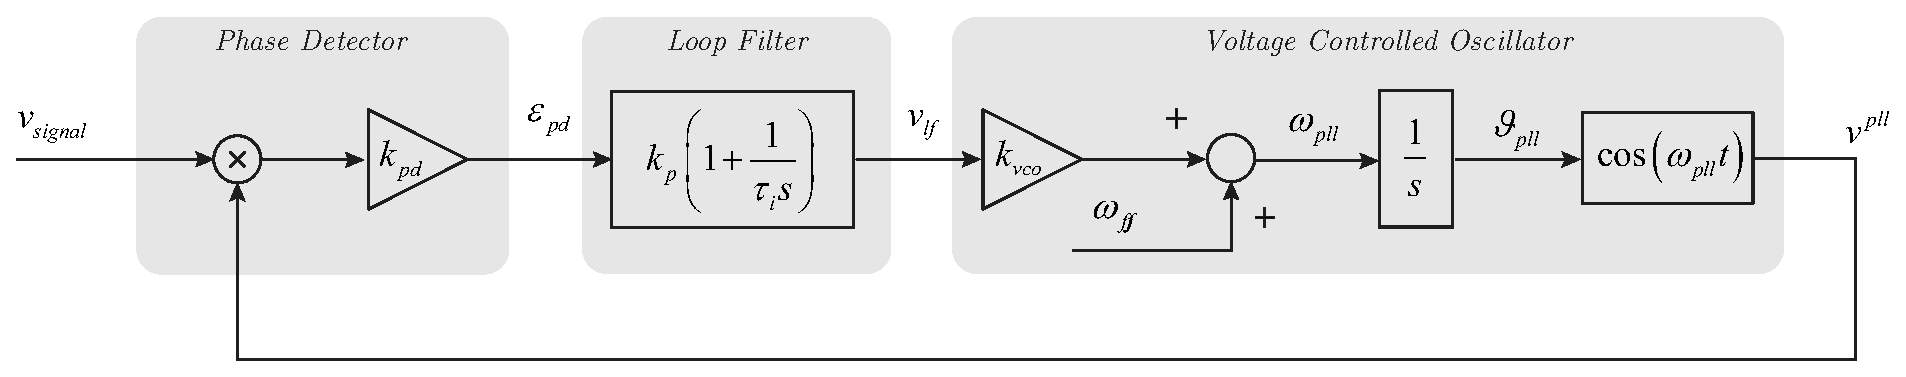
\includegraphics[width=0.95\textwidth]{figures/basic_pll_2.eps}
	\caption{Elementary PLL (figure of rev.~00): multiplier phase detector, PI loop filter, oscillator around the central frequency $\omega\ped{ff}$; $\vartheta\ped{pll}$ is the angle $\theta$ of this note.}
	\label{fig:basic}
\end{figure}

With the multiplier phase detector of Figure~\ref{fig:basic}, an input $v = V\sin\vartheta$ and the oscillator output $v^{pll} = \cos\vartheta\ped{pll}$ give
\begin{equation}
	\varepsilon\ped{pd} = V k\ped{pd} \sin\vartheta \cos\vartheta\ped{pll} = \frac{V k\ped{pd}}{2}\Big[\sin(\vartheta - \vartheta\ped{pll}) + \sin(\vartheta + \vartheta\ped{pll})\Big].
	\label{eq:mult}
\end{equation}
The first term is the phase information, $\approx (V k\ped{pd}/2)(\vartheta - \vartheta\ped{pll})$ near the lock; the second oscillates at twice the grid frequency and is as large as the first. The loop filter has to remove it, and this limits the bandwidth: this double-frequency term is the problem of every single-phase PLL. Linearized (Figure~\ref{fig:basic_ss}), with the PI $k\ped{p}(1 + 1/(\tau\ped{i}s))$ and the oscillator gain $k\ped{vco}$, the loop is
\begin{equation}
	\begin{gathered}
	H(s) = \frac{V k\ped{pd} k\ped{vco}}{2}\,\frac{k\ped{p} s + k\ped{p}/\tau\ped{i}}{s^2}, \\
	H_\vartheta(s) = \frac{\vartheta\ped{pll}}{\vartheta} = \frac{H(s)}{1 + H(s)}, \qquad
	E_\vartheta(s) = \frac{\vartheta - \vartheta\ped{pll}}{\vartheta} = \frac{1}{1 + H(s)},
	\end{gathered}
	\label{eq:basic}
\end{equation}
which are the equations of rev.~00 with $V k\ped{pd} k\ped{vco}/2 = 1$. The two integrators of the open loop let the PLL follow a phase ramp, i.e.\ a frequency step, with no steady-state error; with a proportional loop filter one integrator is left and a frequency step leaves a constant phase error. The gain $V k\ped{pd}/2$ of the detector is part of the loop gain: unless the detector is normalized, the dynamics change with the amplitude of the voltage.

\begin{figure}[H]
	\centering
	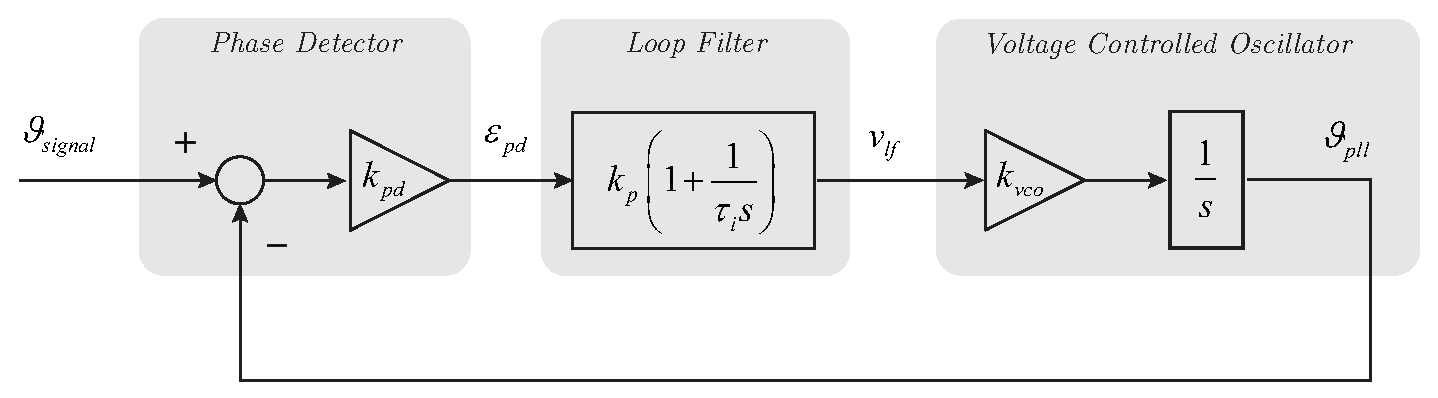
\includegraphics[width=0.7\textwidth]{figures/basic_pll_3.eps}
	\caption{Small-signal model of the elementary PLL (figure of rev.~00).}
	\label{fig:basic_ss}
\end{figure}

The cure for the double-frequency term is a second signal in quadrature with the input. If $u = V\cos\theta\ped{g}$ comes with $\beta = V\sin\theta\ped{g}$, the Park transform of the pair at the angle $\theta$ of the PLL,
\begin{equation}
	\xi = u\cos\theta + \beta\sin\theta = V\cos(\theta\ped{g} - \theta), \qquad \eta = -u\sin\theta + \beta\cos\theta = V\sin(\theta\ped{g} - \theta),
	\label{eq:park}
\end{equation}
gives the phase information with no double-frequency term: the three loops of the model use this ``Park'' phase detector on $\eta$. The quadrature generator that builds $\beta$ is the subject of Section~\ref{sec:qsg}. In the model the oscillator works in pu of the nominal pulsation $\omega_0$: $\dot\theta = \omega_0\,\omega\ped{pu}$, with $\omega\ped{pu} = 1 + k\ped{p}\eta$ in the Park PLL (proportional loop, nominal frequency as feed-forward) and $\omega\ped{pu} = k\ped{p} e + k\ped{i}\int e$ in the other two (the integrator holds the frequency, $e$ the normalized $\eta$). Near the lock the open loop is
\begin{equation}
	L(s) = \omega_0\,\frac{k\ped{p} s + k\ped{i}}{s^2}\; K(s),
	\label{eq:Lgen}
\end{equation}
with $K(s)$ the gain of the detector from $\varepsilon = \theta\ped{g} - \theta$ to the input of the PI: $V$ for a Park detector without normalization, \num{1} with normalization, a transfer function when the detector has dynamics in the loop (Section~\ref{sec:models}).

% =============================================================
\section{Quadrature signal generators}
\label{sec:qsg}

\subsection{Complex gain}
\label{sec:cgain}

A quadrature signal generator (QSG) is a linear system with one input $u$ and two outputs $(\alpha, \beta)$, with the transfer functions $H_\alpha(s) = \alpha/u$ and $H_\beta(s) = \beta/u$. For an input $u = \cos\nu t$ at any frequency $\nu$, the vector $\alpha + j\beta$ is the sum of two rotating components,
\begin{equation}
	\alpha + j\beta = G(\nu)\, e^{j\nu t} + G(-\nu)\, e^{-j\nu t}, \qquad G(\nu) = \tfrac{1}{2}\big(H_\alpha(j\nu) + j H_\beta(j\nu)\big),
	\label{eq:cgain}
\end{equation}
where $\nu$ can be positive or negative. $G$ is the \emph{complex gain} of the generator. An ideal QSG at $\omega_0$ has $G(\omega_0) = 1$ and $G(-\omega_0) = 0$: the input $\cos(\omega_0 t + \varphi)$ becomes the vector $e^{j(\omega_0 t + \varphi)}$, whose angle is the angle of the fundamental. Everything else is an error that the PLL sees, in its frame $e^{-j\theta}$ with $\theta \approx \omega_0 t$:
\begin{itemize}[nosep]
	\item $\angle G(\omega_0) \neq 0$: the vector leads the input by $\angle G(\omega_0)$ and the PLL locks with that offset;
	\item $G(-\omega_0) \neq 0$ (the \emph{image}): a component $e^{-j\omega_0 t}$, which turns at $-2\omega_0$ in the frame: a ripple at \SI{100}{\hertz} on $\eta$;
	\item a DC offset $d$ of the input: $\alpha + j\beta$ gets the constant $2G(0)\,d$, which turns at $-\omega_0$ in the frame: a ripple at \SI{50}{\hertz};
	\item a harmonic $h$: the components $G(h\omega_0)$ and $G(-h\omega_0)$, at $(h-1)\,\omega_0$ and $-(h+1)\,\omega_0$ in the frame;
	\item a frequency off the tuning of a generator with fixed tuning: $\angle G(\omega\ped{g}) \neq 0$ and $G(-\omega\ped{g}) \neq 0$.
\end{itemize}
Each component $c\,e^{jWt}$ of the frame vector, relative to the fundamental, adds $\operatorname{Im}(c\,e^{jWt})$ to the phase error that the detector \eqref{eq:park} reports (Section~\ref{sec:ripple}). Table~\ref{tab:qsg} gives these numbers for the generators of this note.

\subsection{SOGI}
\label{sec:sogi}

The second order generalized integrator (Figure~\ref{fig:sogi}) \cite{ciobotaru2006, teodorescu2011} has
\begin{equation}
	\begin{gathered}
	D(s) = \frac{\alpha}{u} = \frac{k\omega s}{s^2 + k\omega s + \omega^2}, \qquad
	Q(s) = \frac{\beta}{u} = \frac{k\omega^2}{s^2 + k\omega s + \omega^2}, \\
	E(s) = \frac{u - \alpha}{u} = \frac{s^2 + \omega^2}{s^2 + k\omega s + \omega^2},
	\end{gathered}
	\label{eq:sogi}
\end{equation}
a band-pass, a low-pass and a notch at the tuning frequency $\omega$, with the gain $k$ setting the width (and the settling time, about $2/(k\omega)$ for the envelope). Its complex gain is
\begin{equation}
	\begin{gathered}
	G\ped{sogi}(\nu) = \tfrac{1}{2}\big(D(j\nu) + jQ(j\nu)\big) = \frac{j k\omega\,(\omega + \nu)}{2\,(\omega^2 - \nu^2 + j k\omega\nu)}, \\
	G\ped{sogi}(\omega) = 1, \qquad G\ped{sogi}(-\omega) = 0, \qquad |2G\ped{sogi}(0)| = k,
	\end{gathered}
	\label{eq:Gsogi}
\end{equation}
exact at its tuning frequency, and selective: a harmonic $h$ passes with $k(h \pm 1)/(2|1 - h^2 \pm jkh|)$, a DC offset with $k$.

\begin{figure}[H]
	\centering
	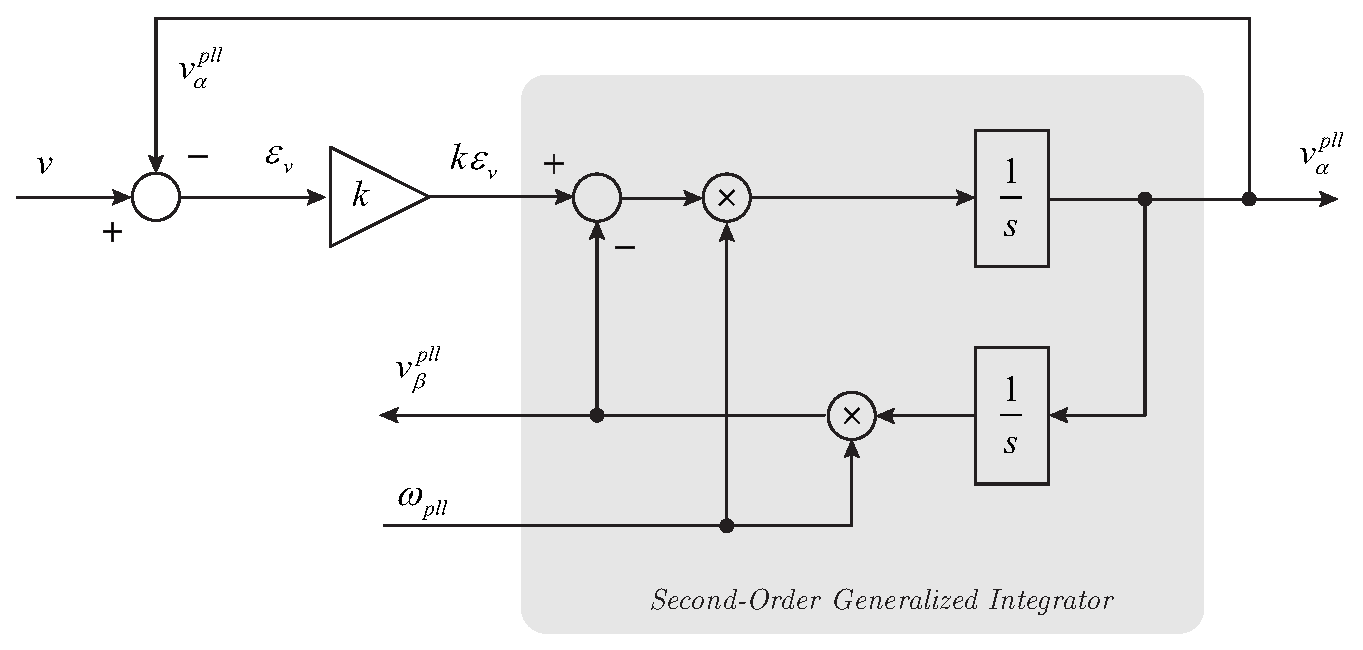
\includegraphics[width=0.7\textwidth]{figures/sogi_1.eps}
	\caption{SOGI quadrature signal generator (figure of rev.~00): $v$ is the input $u$, $v_\alpha^{pll}$ and $v_\beta^{pll}$ are $\alpha$ and $\beta$, $\omega\ped{pll}$ the tuning frequency $\omega$.}
	\label{fig:sogi}
\end{figure}

Rev.~00 derived the band-pass from an adaptive filter, two integrators in a frame turning at $\omega$: the input $g$ is multiplied by $\cos\omega t$ and $\sin\omega t$, integrated and multiplied back. In complex form the filter computes $v = \operatorname{Re}\big\{e^{j\omega t}\int g\,e^{-j\omega t}\,dt\big\}$, and with the shift theorem
\begin{equation}
	V(s) = \frac{1}{2}\Big(\frac{1}{s - j\omega} + \frac{1}{s + j\omega}\Big)\, G(s) = \frac{s}{s^2 + \omega^2}\, G(s),
	\label{eq:af}
\end{equation}
the resonant integrator of rev.~00; closed with the gain $k$ around it, it gives $D(s)$ (with $k\omega$ in place of $k$). The same rotation, filtering and rotation back, with low-pass filters instead of integrators, is the Park generator of the model.

\subsection{The Park generator of the model}
\label{sec:parkqsg}

The block \code{single\_phase\_pll} rotates the pair $(u, \beta)$ by the angle $\theta$ of the PLL (direct Park transform), filters $\xi$ and $\eta$ with two equal low-pass filters $F(s) = \omega\ped{f}/(s + \omega\ped{f})$ and rotates the filtered pair back (inverse Park transform); the $\beta$ of the inverse transform closes the loop on the input of the direct one. In complex form, with $z = u + j\beta$:
\begin{equation}
	x = z\, e^{-j\theta}, \qquad y = F(s)\, x, \qquad w = y\, e^{j\theta} = \hat\alpha + j\beta .
\end{equation}
For $\theta = \omega t$ the rotation, the filter and the rotation back are the filter shifted in frequency, $w = F(s - j\omega)\, z$, i.e.\ $(s - j\omega + \omega\ped{f})\, w = \omega\ped{f}\, z$. Split into real and imaginary parts with $z = u + j\beta$:
\begin{equation}
	(s + \omega\ped{f})\,\hat\alpha + \omega\beta = \omega\ped{f}\, u, \quad s\beta = \omega\hat\alpha
	\quad\Longrightarrow\quad
	\frac{\hat\alpha}{u} = \frac{\omega\ped{f}\, s}{s^2 + \omega\ped{f} s + \omega^2}, \qquad
	\frac{\beta}{u} = \frac{\omega\ped{f}\,\omega}{s^2 + \omega\ped{f} s + \omega^2}:
	\label{eq:parkqsg}
\end{equation}
the transfer functions of rev.~00 (Figure~\ref{fig:parkeq}), and those of a SOGI \eqref{eq:sogi} with $k = \omega\ped{f}/\omega$. The model uses $\tau = 2/\omega_0$, so $\omega\ped{f} = \omega_0/2$ and $k = 0.5$: a narrower and slower SOGI than the $k = \sqrt2$ usual in the literature \cite{ciobotaru2006}, with an envelope time constant of $2/(k\omega_0) = \SI{12.7}{\milli\second}$. Two properties come from the rotation by the angle of the PLL itself. The generator is tuned at every step at the frequency of the PLL: it is frequency adaptive. And it is inside the phase loop: a phase error of the PLL moves the filter states, which live in its frame (Section~\ref{sec:parkmodel}).

\begin{figure}[H]
	\centering
	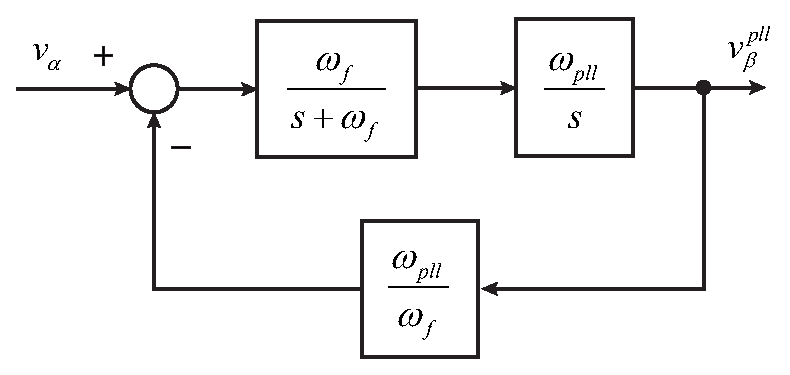
\includegraphics[width=0.42\textwidth]{figures/qsg_park_eq_1.eps}
	\caption{Equivalent diagram of the Park generator (figure of rev.~00): $v_\alpha$ is $u$, $v_\beta^{pll}$ is $\beta$, $\omega_f = 1/\tau$; the signal between the two blocks is $\hat\alpha$.}
	\label{fig:parkeq}
\end{figure}

\paragraph{The detector reads the raw input.} The phase detector of the block is the direct Park transform of the generator, which takes $u$, not $\hat\alpha$: $\eta = -u\sin\theta + \beta\cos\theta$. The vector seen by the detector is $z = u + j\beta$, with the complex gain
\begin{equation}
	G\ped{park}(\nu) = \tfrac{1}{2}\big(1 + jQ(j\nu)\big), \qquad G\ped{park}(\omega_0) = 1, \quad G\ped{park}(-\omega_0) = 0, \quad |2G\ped{park}(0)| = |1 + jk| = 1.12 .
	\label{eq:Gpark}
\end{equation}
It is exact at the tuning frequency, but every other component of $u$ reaches the detector directly: $Q$ is small away from $\omega_0$ and $|G\ped{park}(\pm h\omega_0)| \approx 0.5$ for the harmonics (Table~\ref{tab:qsg}). The filtered $\eta\ped{f} = \operatorname{Im} y$, which the block also computes (\code{ueta\_pll\_flt}), is $\operatorname{Im}\{(\hat\alpha + j\beta)e^{-j\theta}\}$: the detector of the SOGI-PLL of the literature, which rotates the outputs $(\hat\alpha, \beta)$ of the generator (Figure~\ref{fig:sogipll}), with the complex gain $G\ped{sogi}$ of \eqref{eq:Gsogi}. The PI of the model reads $\eta$, so the harmonics bypass the generator; reading $\eta\ped{f}$ is a one-line change with a price (Section~\ref{sec:critpark}).

\begin{figure}[H]
	\centering
	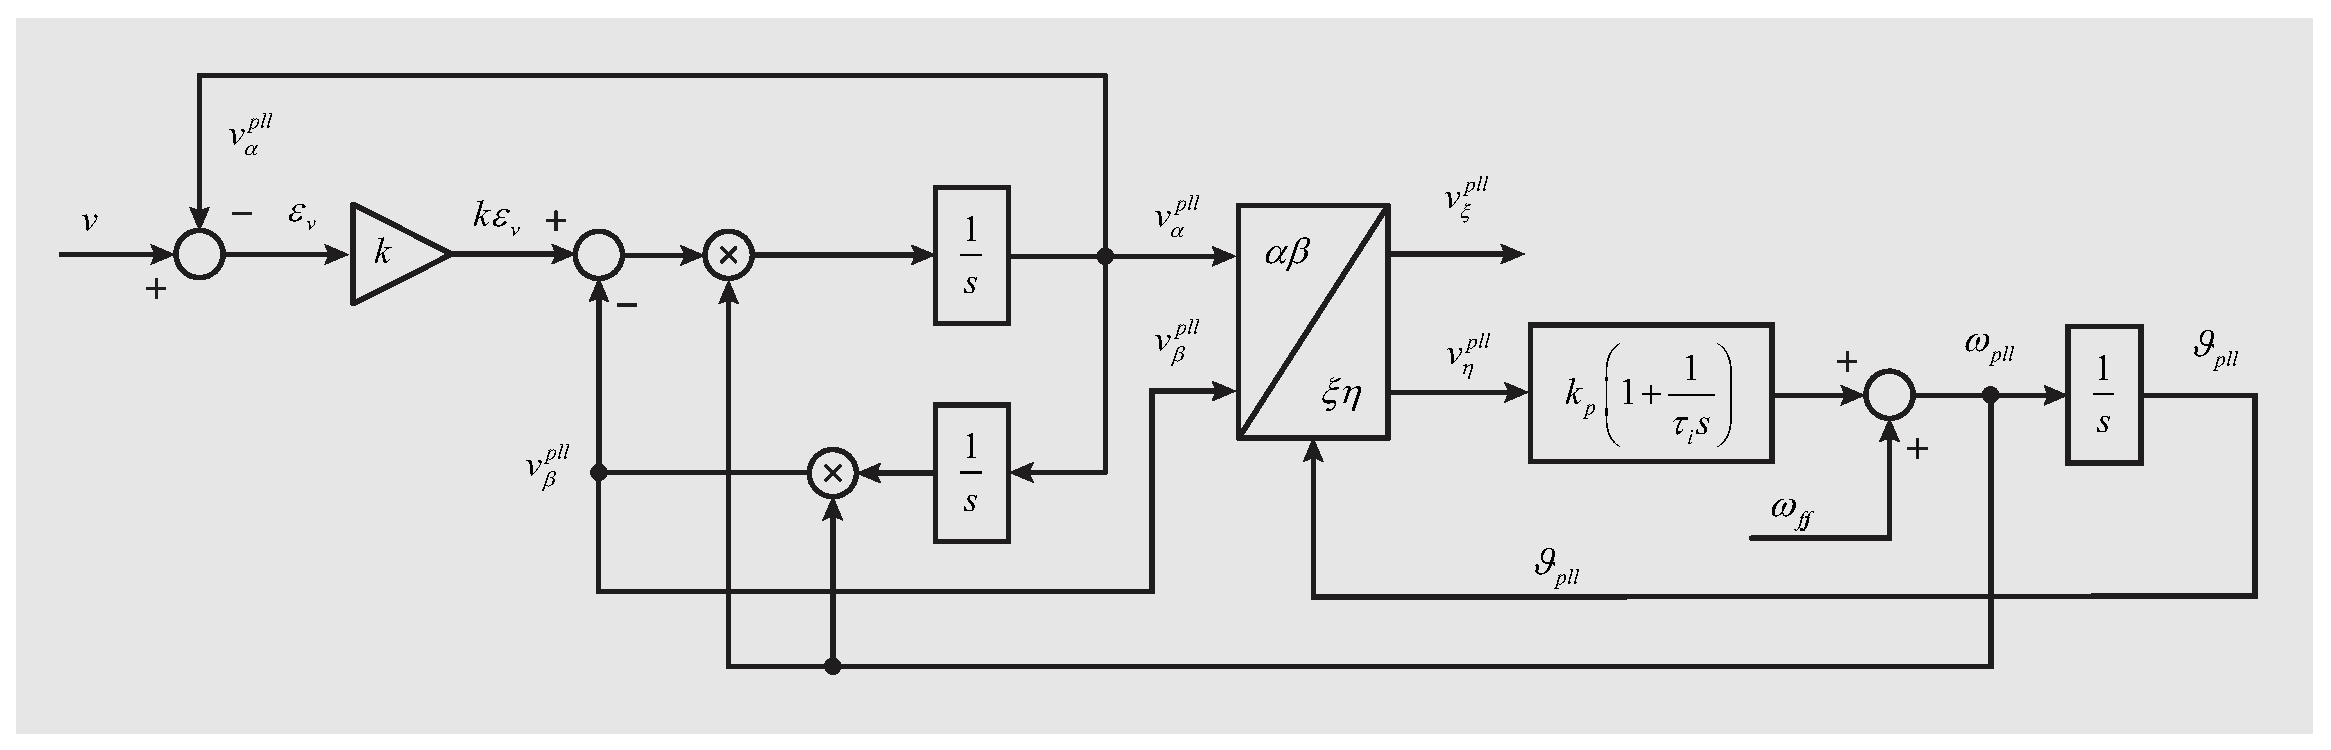
\includegraphics[width=0.95\textwidth]{figures/sogi_pll_2.eps}
	\caption{SOGI-PLL (figure of rev.~00): the Park transform reads the outputs $v_\alpha^{pll}$, $v_\beta^{pll}$ of the SOGI. In the Park PLL of the model the SOGI is built with Park transforms at $\vartheta\ped{pll}$ (Figure~\ref{fig:parkpll}) and the detector reads the raw input in place of $v_\alpha^{pll}$.}
	\label{fig:sogipll}
\end{figure}

\subsection{The first harmonic tracker}
\label{sec:fht}

The first harmonic tracker of the library (class \code{ctrl\_afe\_setup}, parameters \code{fht\_grid}) is a Luenberger observer of a damped harmonic oscillator at $\omega_0$, with the input $u$ as the measurement of the first state:
\begin{equation}
	\dot x = A x + L\,(u - x_1), \qquad A = \begin{bmatrix} 0 & 1 \\ -\omega_0^2 & -\delta\omega_0 \end{bmatrix}, \qquad \alpha = x_1, \quad \beta = -x_2/\omega_0,
	\label{eq:fht}
\end{equation}
with $\delta = 0.05$ ($\beta = \sin$ for $u = \cos$). The model computes it as $x[k+1] = A\ped{d}\,x[k] + L\ped{d}\,(u[k] - x_1[k])$, with the forward Euler matrix $A\ped{d} = I + A t\ped{s}$ and the gains $L\ped{d} = [0.18191,\ 29.588]^T$ placed by Ackermann's formula at $e^{-\omega_0 t\ped{s}}$ and $e^{-4\omega_0 t\ped{s}}$; the outputs of step $k$ are the states $x[k]$, predicted at step $k-1$. The continuous equivalent has the poles $-\omega_0$ and $-4\omega_0$ (\SI{3.2}{} and \SI{0.8}{\milli\second}), $l_1 = 4.95\,\omega_0$, $l_2 = 2.7525\,\omega_0^2$, and the transfer functions
\begin{equation}
	H_1(s) = \frac{x_1}{u} = \frac{l_1 s + l_1\delta\omega_0 + l_2}{\Delta(s)}, \qquad
	H_2(s) = \frac{x_2/\omega_0}{u} = \frac{l_2 s - l_1\omega_0^2}{\omega_0\,\Delta(s)}, \qquad
	\Delta(s) = (s + \omega_0)(s + 4\omega_0),
	\label{eq:H12}
\end{equation}
so that $G\ped{fht}(\nu) = \tfrac12\big(H_1(j\nu) - jH_2(j\nu)\big)$. The tracker is a generalization of the SOGI: with $\delta = 0$ and $l_2 = 0$, $H_1 = l_1 s/(s^2 + l_1 s + \omega_0^2)$ and $-H_2 = l_1\omega_0/(s^2 + l_1 s + \omega_0^2)$ are $D$ and $Q$ with $k = l_1/\omega_0$. For poles $p_1$, $p_2$ (with $\delta = 0$) the gains are $l_1 = -(p_1 + p_2)$, $l_2 = p_1 p_2 - \omega_0^2$, and the DC gain of $\alpha$ is $H_1(0) = 1 - \omega_0^2/(p_1 p_2)$: zero for the SOGI ($|p| = \omega_0$), $3/4$ for the poles of the model. These poles make the tracker fast and wide: $|2G\ped{fht}(0)| = 1.47$ and the harmonics on the positive side pass with \num{0.4} to \num{0.9} (Table~\ref{tab:qsg}). It is a fast estimator of the fundamental, not a selective filter.

\paragraph{The error at \SI{50}{\hertz}.} The tracker is not exact at its own tuning frequency: $G\ped{fht}(\omega_0) = 0.9959\angle\ang{0.74}$ with an image of \num{0.0142}. The observer can only be exact on a signal its internal model contains, and the model of the class is a damped oscillator, discretized by forward Euler: the eigenvalues of $I + A t\ped{s}$ have the modulus \num{0.999789}, a damping of \SI{-1.686}{\per\second} (the continuous model has $-\delta\omega_0/2 = \SI{-7.854}{\per\second}$, and forward Euler removes about \num{80}~\% of it). In both forms the mode of the model is not the undamped \SI{50}{\hertz} of the input, and the estimation error does not vanish. With the undamped oscillator and the exact discretization $A\ped{d} = e^{A t\ped{s}}$, $\delta = 0$ (option \code{param.afe.pll.fht\_undamped} of the init, $L\ped{d} = [0.18233,\ 31.330]^T$ for the same poles) the internal model contains the \SI{50}{\hertz} mode exactly and the tracker is exact: $G\ped{fht}(\omega_0) = 1$, no image. At \SI{49}{\hertz} both have an error, because the tuning stays at $\omega_0$: \ang{1.61} with an image of \num{0.023} (class) and \ang{0.87} with \num{0.010} (undamped).

\paragraph{The positive-sequence calculator of the FHT-PLL.} The FHT-PLL filters $\alpha$ and $\beta$ of the first tracker with two more trackers and combines their outputs as in the three-phase calculator \cite{note_3ph}, $u\ped{sr} = -\tfrac12(\hat u - j\hat v)$ with $\hat u = \hat u_\alpha + j\hat u_\beta$ (states $x_1$) and $\hat v = \hat v_\alpha + j\hat v_\beta$ (states $x_2/\omega_0$). A component $Z e^{j\nu t}$ of $\alpha + j\beta$ gives $\hat u = H_1(j\nu)\,Z e^{j\nu t}$ and $\hat v = H_2(j\nu)\,Z e^{j\nu t}$, so $u\ped{sr} = -G\ped{fht}(\nu)\,Z e^{j\nu t}$, and stage A of the FHT-PLL has the complex gain
\begin{equation}
	G\ped{A}(\nu) = G\ped{fht}(\nu)^2
	\label{eq:GA}
\end{equation}
(the sign is compensated by a gain $-1$ before the PI). The second stage squares the selectivity (image \num{0.0002}, harmonics \num{0.1} to \num{0.8}) and doubles the angle errors: \ang{1.49} at \SI{50}{\hertz}, \ang{3.22} at \SI{49}{\hertz}.

\subsection{The generators side by side}
\label{sec:qsgcompare}

\begin{table}[H]
	\centering
	\caption{Complex gain of the generators: gain and angle at \SI{50}{\hertz}, image, DC, harmonics (positive / negative side, $|G(\pm h\omega_0)|/|G(\omega_0)|$), angle and image at \SI{49}{\hertz}. Park: the vector $u + j\beta$ of the detector of the model; SOGI $k = 0.5$: $(\hat\alpha, \beta)$ of the same block, the detector $\eta\ped{f}$; the two turn with the PLL and are tuned at its frequency, so the \SI{49}{\hertz} columns do not apply. Trackers: class design ($\delta = 0.05$, forward Euler) and the option \code{fht\_undamped}; stage A: the two trackers in series of the FHT-PLL.}
	\label{tab:qsg}
	\footnotesize
	\setlength{\tabcolsep}{3.5pt}
	\rowcolors{3}{tableShade}{white}
	\resizebox{\textwidth}{!}{%
	\begin{tabular}{@{} l c c c c c c c c c c @{}}
		\toprule
		 & \multicolumn{3}{c}{\SI{50}{\hertz}} & DC & \multicolumn{4}{c}{harmonics $h$, $+/-$} & \multicolumn{2}{c@{}}{\SI{49}{\hertz}} \\
		generator & $|G|$ & angle & image & $|2G(0)|$ & 2 & 3 & 5 & 7 & angle & image \\
		\midrule
		Park, $u + j\beta$ & 1.0000 & \ang{0.00} & 0.0000 & 1.12 & 0.53/0.48 & 0.51/0.50 & 0.50/0.50 & 0.50/0.50 & adaptive & -- \\
		SOGI $k = 0.5$, $\hat\alpha + j\beta$ & 1.0000 & \ang{0.00} & 0.0000 & 0.50 & 0.24/0.08 & 0.12/0.06 & 0.06/0.04 & 0.04/0.03 & adaptive & -- \\
		FHT, class & 0.9959 & \ang{0.74} & 0.0142 & 1.47 & 0.87/0.28 & 0.73/0.36 & 0.53/0.35 & 0.41/0.30 & \ang{1.61} & 0.0228 \\
		FHT, undamped & 1.0000 & \ang{0.00} & 0.0000 & 1.46 & 0.87/0.29 & 0.74/0.37 & 0.54/0.36 & 0.41/0.31 & \ang{0.87} & 0.0101 \\
		stage A, class & 0.9918 & \ang{1.49} & 0.0002 & 1.09 & 0.76/0.08 & 0.54/0.13 & 0.28/0.12 & 0.17/0.09 & \ang{3.22} & 0.0005 \\
		stage A, undamped & 1.0000 & \ang{0.00} & 0.0000 & 1.06 & 0.77/0.09 & 0.54/0.14 & 0.29/0.13 & 0.17/0.09 & \ang{1.74} & 0.0001 \\
		\bottomrule
	\end{tabular}}
	\rowcolors{1}{white}{white}
\end{table}

\begin{figure}[H]
	\centering
	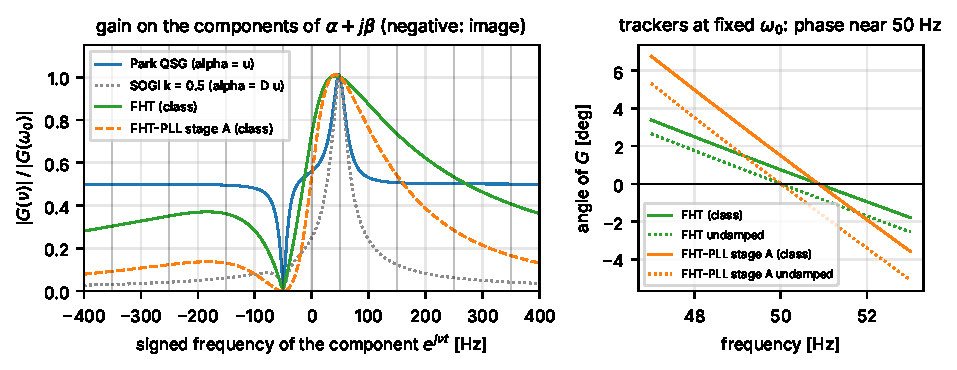
\includegraphics[width=\textwidth]{figures/qsg_gains.pdf}
	\caption{Left: gain $|G(\nu)|/|G(\omega_0)|$ of the generators on a component $e^{j\nu t}$ of the input (negative frequencies: image side). Right: angle of $G$ near \SI{50}{\hertz} for the trackers, class design and undamped; the Park generator follows the PLL frequency and is not shown.}
	\label{fig:qsg}
\end{figure}

The table puts the three generators in order of selectivity. The detector of the Park PLL is the least selective, because the raw input reaches it: half of every harmonic on both sides, \num{1.12} of a DC offset. The single tracker of the DDSRF-PLL lets through more of the positive side (\num{0.4} to \num{0.9}) but less of the negative one, and has the error at \SI{50}{\hertz} of its design. Stage A of the FHT-PLL is the most selective of the three as built, with twice the angle error. The SOGI with $k = 0.5$, which the Park block already computes, is the most selective of all on harmonics and DC.

% =============================================================
\section{The model and its three PLLs}
\label{sec:model}

\subsection{Test bench and test cases}
\label{sec:bench}

The model is discrete with a fixed step equal to the control period $t\ped{s} = \SI{125}{\micro\second}$ and runs for \SI{1}{\second} (Figure~\ref{fig:bench}). The block \code{test\_signal} (MATLAB Function, mask parameter \code{p = param.test}) computes every $t\ped{s}$
\begin{equation}
	u = A(t)\Big(\cos(\phi + \theta_0) + \sum_h a_h \sin(h\phi + \varphi_h)\Big) + d(t), \qquad \theta\ped{g} = \wrapop(\phi + \theta_0), \qquad \dot\phi = \omega_0\,\omega\ped{g},
	\label{eq:testsig}
\end{equation}
with the phase jump added to $\phi$, the frequency step in $\omega\ped{g}$ (pu), the amplitude $A(t)$ stepping for the sag and the DC offset $d(t)$. The six cases of \code{private/test\_param.m} are in Table~\ref{tab:cases}; case 1 is the test signal of the 2021 model. The three PLLs read $u$; the To Workspace blocks of \code{data\_logging} keep $[t,\ u,\ \theta\ped{g},\ \omega\ped{g}]$ and the angle and frequency of each PLL, one row per control period.

\begin{figure}[H]
	\centering
	\begin{tikzpicture}[font=\scriptsize, >=Latex,
		blk/.style={draw, thick, rounded corners=2pt, fill=orange!15, minimum width=2.6cm, minimum height=0.8cm, align=center},
		sm/.style={draw, thick, rounded corners=2pt, fill=gray!12, minimum width=2.4cm, minimum height=0.8cm, align=center}]
		\node[sm] (ts) at (0,0) {\code{test\_signal}\\$p = $ \code{param.test}};
		\node[blk] (p1) at (4.2,1.1) {Park PLL\\\code{single\_phase\_pll}};
		\node[blk] (p2) at (4.2,0) {FHT-PLL};
		\node[blk] (p3) at (4.2,-1.1) {DDSRF-PLL};
		\node[sm, minimum height=3.0cm] (log) at (8.4,0) {\code{data\_logging}\\[2pt]\code{sig\_log}\\\code{park\_pll\_log}\\\code{fht\_pll\_log}\\\code{ddsrf\_pll\_log}};
		\draw[->] (ts.east) -- node[above, pos=0.2] {$u$} (p2.west);
		\draw[->] (2.2,0) |- (p1.west);
		\draw[->] (2.2,0) |- (p3.west);
		\fill (2.2,0) circle (1.2pt);
		\draw[->] (p1.east) -- node[above] {$\theta\ped{out}$, $\omega\ped{pu}$} (log.west |- p1.east);
		\draw[->] (p2.east) -- node[above] {$\theta\ped{out}$, $\omega\ped{pu}$} (log.west |- p2.east);
		\draw[->] (p3.east) -- node[above] {$\theta\ped{out}$, $\omega\ped{pu}$} (log.west |- p3.east);
		\draw[->] (ts.south) |- node[pos=0.75, below] {$u$, $\theta\ped{g}$, $\omega\ped{g}$} (8.4,-2.0) -- (log.south);
	\end{tikzpicture}
	\caption{The test bench \code{single\_phase\_pll\_analysis.slx}: one test signal, three PLLs, logging at $t\ped{s}$.}
	\label{fig:bench}
\end{figure}

\begin{table}[H]
	\centering
	\caption{Test cases of the model (\code{param.sim.test\_case}, \code{private/test\_param.m}); an event not listed is off.}
	\label{tab:cases}
	\footnotesize
	\rowcolors{2}{tableShade}{white}
	\begin{tabularx}{\textwidth}{@{} c X @{}}
		\toprule
		case & test signal \\
		\midrule
		1 & the 2021 model: 4th and 5th harmonic \SI{10}{\percent}, sag to \num{0.2} pu from \SI{0.25}{} to \SI{0.5}{\second}, start \ang{180} away from the PLLs \\
		2 & phase jump of \ang{+30} at \SI{0.4}{\second} \\
		3 & frequency step from \SI{50}{} to \SI{49}{\hertz} at \SI{0.4}{\second} \\
		4 & DC offset of \num{0.02} pu from \SI{0.4}{\second} \\
		5 & odd harmonics from \SI{0}{\second}: 3rd \SI{5}{\percent}, 5th \SI{6}{\percent}, 7th \SI{5}{\percent} (the limits of EN 50160 \cite{en50160}) \\
		6 & sag to \num{0.2} pu from \SI{0.25}{} to \SI{0.5}{\second}, no harmonics \\
		\bottomrule
	\end{tabularx}
	\rowcolors{1}{white}{white}
\end{table}

The metrics of \code{private/pll\_metrics.m} use the phase error $e_\theta = \theta\ped{out} - \theta\ped{g}$ wrapped to $(-\ang{180}, \ang{180}]$: the \emph{lock time} (first time after which $|e_\theta| < \ang{5}$ until the first event), the \emph{offset} (mean of $e_\theta$ in the \SI{0.1}{\second} before the event), the \emph{peak} (largest $|e_\theta - \text{offset}|$ after the event), the \emph{settling time} (from the event until $e_\theta$ stays within \ang{1} of its final mean), the \emph{final error} and the \emph{ripple} (mean and peak to peak in the last \SI{0.2}{\second}).

\subsection{Park PLL}
\label{sec:parkpll}

Figure~\ref{fig:parkpll} shows the block \code{single\_phase\_pll}. At step $k$, with $\theta[k]$ the state of the angle integrator and $y_\xi[k]$, $y_\eta[k]$ the outputs of the two filters (the library block \code{discrete\_time\_low\_pass\_filter}, no feedthrough):
\begin{align}
	\beta[k] &= y_\xi[k]\sin\theta[k] + y_\eta[k]\cos\theta[k], \notag \\
	\xi[k] &= u[k]\cos\theta[k] + \beta[k]\sin\theta[k], \qquad \eta[k] = -u[k]\sin\theta[k] + \beta[k]\cos\theta[k], \notag \\
	y[k+1] &= y[k] + \frac{t\ped{s}}{\tau}\big(x[k] - y[k]\big) \quad \text{for } (x, y) = (\xi, y_\xi),\ (\eta, y_\eta), \label{eq:parkblock} \\
	\omega\ped{pu}[k] &= 1 + \sat_{\pm 2}\big(k\ped{p}\eta[k] + i[k]\big), \qquad \theta[k+1] = \wrapop\big(\theta[k] + \omega_0 t\ped{s}\, \omega\ped{pu}[k]\big), \notag
\end{align}
where $i$ is the integrator of the block \code{pi-ctrl} (back-calculation on the saturation; idle with $k\ped{i} = 0$). The parameters are in \code{param.afe.pll.park}: $\tau = 2/\omega_0$ ($k = 0.5$), $k\ped{p} = 1$, $k\ped{i} = 0$, limits $\pm 2$ pu around the nominal frequency. The error $\eta$ is not normalized. The outputs of the block are the angle $\hat\theta$ and the frequency $\hat\omega$ of the double-integrator observer of Section~\ref{sec:obs}, fed with $\theta$.

\begin{figure}[H]
	\centering
	\begin{tikzpicture}[font=\scriptsize, >=Latex,
		blk/.style={draw, thick, rounded corners=2pt, fill=orange!15, minimum width=2.0cm, minimum height=1.0cm, align=center},
		sm/.style={draw, thick, rounded corners=2pt, fill=gray!12, minimum width=1.3cm, minimum height=0.6cm, align=center},
		sumn/.style={draw, thick, circle, minimum size=0.35cm, inner sep=0pt}]
		% quadrature generator
		\node[blk] (pk) at (0,0) {direct Park\\at $\theta$};
		\node[sm] (fx) at (2.7,0.6) {$F(s)$};
		\node[sm] (fe) at (2.7,-0.6) {$F(s)$};
		\node[blk] (ipk) at (6.0,0) {inverse Park\\at $\theta$};
		\draw[->] (-2.3,0.25) node[left] {$u$} -- ($(pk.west)+(0,0.25)$);
		\draw[->] ($(pk.east)+(0,0.25)$) -- ++(0.45,0) |- node[pos=0.75, above] {$\xi$} (fx.west);
		\draw[->] ($(pk.east)+(0,-0.25)$) -- ++(0.45,0) |- node[pos=0.75, below] {$\eta$} (fe.west);
		\draw[->] (fx.east) -- node[above] {$y_\xi$} ++(1.1,0) |- ($(ipk.west)+(0,0.25)$);
		\draw[->] (fe.east) -- node[below] {$y_\eta = \eta\ped{f}$} ++(1.1,0) |- ($(ipk.west)+(0,-0.25)$);
		\draw[->, dashed] ($(ipk.east)+(0,0.25)$) -- ++(0.6,0) node[right] {$\hat\alpha$ (not used)};
		\draw[->] (ipk.north) -- ++(0,0.75) -| node[pos=0.25, above] {$\beta$} (-1.6,-0.25) -- ($(pk.west)+(0,-0.25)$);
		% loop
		\node[sm] (pi) at (2.7,-2.3) {PI $k\ped{p}$, $k\ped{i}$\\sat $\pm 2$};
		\node[sumn] (sm1) at (4.5,-2.3) {$+$};
		\node[sm] (int) at (6.3,-2.3) {$\dfrac{\omega_0 t\ped{s}}{z-1}$, wrap};
		\node[sm] (obs) at (9.5,-2.3) {DI observer};
		\draw[->] (1.2,-0.25) |- (pi.west);
		\fill (1.2,-0.25) circle (1.2pt);
		\draw[->] (pi.east) -- (sm1.west);
		\draw[->] (4.5,-1.55) node[above] {$1$ pu} -- (sm1.north);
		\draw[->] (sm1.east) -- node[above] {$\omega\ped{pu}$} (int.west);
		\draw[->] (int.east) -- node[above, pos=0.3] {$\theta$} (obs.west);
		\draw[->] (obs.east) -- ++(0.5,0.25) node[right] {$\theta\ped{out} = \hat\theta$};
		\draw[->] (obs.east) -- ++(0.5,-0.25) node[right] {$\omega\ped{pu} = \hat\omega/\omega_0$};
		\draw[->] (8.1,-2.3) -- (8.1,-1.3) -| (ipk.south);
		\draw[->] (8.1,-2.3) -- (8.1,-3.2) -| (pk.south);
		\fill (8.1,-2.3) circle (1.2pt);
		\draw[->, dashed] (fe.south) -- ++(0,-0.75) node[right, pos=0.6] {variant} -| ($(pi.north)+(0.3,0)$);
		\node[font=\tiny, anchor=north] at (4.0,-3.25) {$\theta$ (one step late)};
	\end{tikzpicture}
	\caption{Park PLL (block \code{single\_phase\_pll}). The direct Park transform, the two filters $F(s) = \omega\ped{f}/(s+\omega\ped{f})$ and the inverse Park transform are the quadrature generator; the direct transform is also the phase detector, on the raw $u$. Dashed: the filtered $\eta\ped{f}$, the detector of the SOGI-PLL, as variant input of the PI (Section~\ref{sec:critpark}).}
	\label{fig:parkpll}
\end{figure}

\subsection{FHT-PLL}
\label{sec:fhtpll}

Stage A of the FHT-PLL (Figure~\ref{fig:fhtpll}) is the first tracker on $u$, which gives $(\alpha, \beta) = (x_1, -x_2/\omega_0)$, the two trackers on $\alpha$ and on $\beta$ and the calculator $u\ped{sr} = -\tfrac12(\hat u - j\hat v)$ of Section~\ref{sec:fht}, the normalization $V\ped{norm} = 1/\sqrt{\max(|u\ped{sr}|^2,\, 0.02)}$ and the rotation by $\theta$. Stage B, the block \code{pll\_stageB} of the library, is the loop:
\begin{align}
	e[k] &= -\eta[k]\, V\ped{norm}[k], \qquad i[k] = i[k-1] + k\ped{i} t\ped{s}\, e[k], \qquad \omega\ped{pu}[k] = k\ped{p} e[k] + i[k], \notag \\
	\theta[k+1] &= \wrapop\big(\theta[k] + \omega_0 t\ped{s}\, \omega\ped{pu}[k]\big),
	\label{eq:stageB}
\end{align}
with the gains of the class, \code{pll\_p\_fht} $= 1$ and \code{pll\_i1\_fht} $= 80$, no clamp and the integrator starting at zero. The block gives the angle $\theta\ped{out}[k] = \theta[k]$ (unit delay) and the frequency of the double-integrator observer. The three trackers are linear filters of $u$ alone: they do not see $\theta$, and they are outside the loop.

\begin{figure}[H]
	\centering
	\begin{tikzpicture}[font=\scriptsize, >=Latex,
		blk/.style={draw, thick, rounded corners=2pt, fill=orange!15, minimum width=1.8cm, minimum height=0.8cm, align=center},
		sm/.style={draw, thick, rounded corners=2pt, fill=gray!12, minimum width=1.3cm, minimum height=0.7cm, align=center}]
		\node[blk] (f1) at (0,0) {FHT\\on $u$};
		\node[blk] (fa) at (2.6,0.75) {FHT on $\alpha$\\$\hat u_\alpha$, $\hat v_\alpha$};
		\node[blk] (fb) at (2.6,-0.75) {FHT on $\beta$\\$\hat u_\beta$, $\hat v_\beta$};
		\node[blk, minimum width=2.5cm] (ps) at (5.5,0) {$u\ped{sr} = -\tfrac12(\hat u - j\hat v)$\\$\times V\ped{norm}$};
		\node[sm] (rot) at (8.0,0) {rotation\\by $-\theta$};
		\node[sm] (sb) at (10.3,0) {stage B\\$\times(-1)$, PI};
		\draw[->] (-1.5,0) node[left] {$u$} -- (f1);
		\draw[->] (f1.east) -- ++(0.3,0) |- node[pos=0.75, above] {$\alpha$} (fa.west);
		\draw[->] (f1.east) -- ++(0.3,0) |- node[pos=0.75, below] {$\beta$} (fb.west);
		\draw[->] (fa.east) -| ($(ps.north west)+(0.3,0)$);
		\draw[->] (fb.east) -| ($(ps.south west)+(0.3,0)$);
		\draw[->] (ps) -- (rot);
		\draw[->] (rot) -- node[above] {$\eta$} (sb);
		\draw[->] (sb.east) -- ++(0.4,0) node[right] {$\theta\ped{out}$, $\omega\ped{pu}$};
		\draw[->] (sb.south) -- ++(0,-0.6) -| node[pos=0.25, below] {$\theta$ (one step late)} (rot.south);
	\end{tikzpicture}
	\caption{FHT-PLL. The three trackers are instances of the same design (parameters \code{fht\_grid}: tuning $\omega_0$, $\delta = 0.05$, gains $L\ped{d}$); stage B is the loop \eqref{eq:stageB} with the observer.}
	\label{fig:fhtpll}
\end{figure}

\subsection{DDSRF-PLL}
\label{sec:ddsrfpll}

The DDSRF-PLL (Figure~\ref{fig:ddsrfpll}) uses one tracker. Its outputs $(\alpha, \beta)$ are normalized with $V\ped{norm} = 1/\sqrt{\max(\alpha^2 + \beta^2,\, 0.02)}$ and feed the decoupled double frame: the vector $v = \alpha + j\beta$ in the positive frame, $x\ped{p} = v\,e^{-j\theta}$, and in the negative frame, $x\ped{n} = v\,e^{j\theta}$, each filtered by two low-pass filters $F$ ($\tau = 1/\omega_0$) after removing the output of the other frame rotated into it:
\begin{equation}
	y\ped{p} = F(s)\big[x\ped{p} - y\ped{n} e^{-j2\theta}\big], \qquad y\ped{n} = F(s)\big[x\ped{n} - y\ped{p} e^{j2\theta}\big].
	\label{eq:ddsrf}
\end{equation}
For $v = V\ped{p}e^{j\theta\ped{g}} + V\ped{n}e^{-j\theta\ped{g}}$ and $\theta = \theta\ped{g}$ the outputs settle at $y\ped{p} = V\ped{p}$, $y\ped{n} = V\ped{n}$: the cross terms cancel the component of the other sequence exactly. Stage B \eqref{eq:stageB} reads $e = \operatorname{Im}(y\ped{p})\,V\ped{norm}$ (no sign change) with $k\ped{p} = 0.32$, $k\ped{i} = 8$ (the gains proposed in \cite{note_3ph} and set in \code{frt\_dqpll}), and a Saturation block clamps the frequency integrator to $[0.5,\ 1.5]$ pu. The integrator starts at zero, so the clamp holds it at \num{0.5} pu from the first step.

\begin{figure}[H]
	\centering
	\begin{tikzpicture}[font=\scriptsize, >=Latex,
		blk/.style={draw, thick, rounded corners=2pt, fill=orange!15, minimum width=1.6cm, minimum height=0.8cm, align=center},
		sm/.style={draw, thick, rounded corners=2pt, fill=gray!12, minimum width=1.2cm, minimum height=0.6cm, align=center},
		sumn/.style={draw, thick, circle, minimum size=0.35cm, inner sep=0pt}]
		\node[blk] (f1) at (0,0) {FHT on $u$\\$\times V\ped{norm}$};
		\node[sm] (rp) at (2.4,1.2) {$e^{-j\theta}$};
		\node[sm] (rn) at (2.4,-1.2) {$e^{+j\theta}$};
		\node[sumn] (sp) at (3.9,1.2) {};
		\node[sumn] (sn) at (3.9,-1.2) {};
		\node[sm] (fp) at (5.3,1.2) {$F(s)$};
		\node[sm] (fn) at (5.3,-1.2) {$F(s)$};
		\node[sm] (cn) at (7.0,0.4) {$e^{-j2\theta}$};
		\node[sm] (cp) at (7.0,-0.4) {$e^{+j2\theta}$};
		\node[sm] (sb) at (10.0,1.2) {$\operatorname{Im}$, stage B\\PI, clamp};
		\draw[->] (-1.5,0) node[left] {$u$} -- (f1);
		\draw[->] (f1.east) -- ++(0.4,0) |- node[pos=0.75, above] {$v$} (rp.west);
		\draw[->] (f1.east) -- ++(0.4,0) |- (rn.west);
		\draw[->] (rp) -- node[above] {$x\ped{p}$} (sp);
		\draw[->] (rn) -- node[below] {$x\ped{n}$} (sn);
		\draw[->] (sp) -- (fp);
		\draw[->] (sn) -- (fn);
		\draw[->] (fp.east) -- node[above, pos=0.3] {$y\ped{p}$} (sb.west);
		\draw (fn.east) -- node[below, pos=0.4] {$y\ped{n}$} (7.9,-1.2);
		\draw[->] (7.9,-1.2) |- (cn.east);
		\draw[->] (8.2,1.2) |- (cp.east);
		\fill (8.2,1.2) circle (1.2pt);
		\draw[->] (cn.west) -| node[pos=0.85, right] {$-$} (sp.south);
		\draw[->] (cp.west) -| node[pos=0.85, right] {$-$} (sn.north);
		\draw[->] (sb.east) -- ++(0.4,0) node[right] {$\theta\ped{out}$, $\omega\ped{pu}$};
		\draw[->] (sb.south) -- ++(0,-3.2) -| node[pos=0.25, below] {$\theta$ (one step late), to the four rotations} (rn.south);
	\end{tikzpicture}
	\caption{DDSRF-PLL: one tracker, normalization, positive and negative frame with the decoupling \eqref{eq:ddsrf} (four filters $F$, $\tau = 1/\omega_0$, on complex pairs), stage B on $\operatorname{Im} y\ped{p}$ with the frequency integrator clamped to $[0.5,\ 1.5]$ pu.}
	\label{fig:ddsrfpll}
\end{figure}

\subsection{Double-integrator observer}
\label{sec:obs}

Each loop ends in the double-integrator observer of the library (\code{di\_obs} of \code{ctrl\_afe\_setup}): $x[k+1] = A\ped{d}\,x[k] + L\ped{dso}\,\wrapop\big(\theta[k] - \wrapop(x_1[k])\big)$, $A\ped{d} = [1,\ t\ped{s};\ 0,\ 1]$, $L\ped{dso} = [0.18387,\ 44.782]^T$ (poles $e^{-\omega_0 t\ped{s}}$, $e^{-4\omega_0 t\ped{s}}$), with the outputs $\hat\theta = \wrapop(x_1)$ and $\hat\omega = x_2$. In continuous time
\begin{equation}
	O(s) = \frac{\hat\theta}{\theta} = \frac{5\omega_0 s + 4\omega_0^2}{s^2 + 5\omega_0 s + 4\omega_0^2},
	\label{eq:obs}
\end{equation}
no error at constant frequency and about \SI{4}{\milli\second} of delay in the transients. The frequency of the three PLLs is $\hat\omega/\omega_0$; the angle is $\hat\theta$ in the Park PLL and $\theta$ in the other two.

% =============================================================
\section{Linear models of the loops}
\label{sec:models}

The three loops differ in where the front end sits with respect to the loop (Figure~\ref{fig:linmodel}): the generator of the Park PLL turns with $\theta$ and is inside the loop; the trackers of the FHT-PLL are outside it; the DDSRF-PLL has its tracker outside and its decoupling network inside. With the loop filter of \eqref{eq:Lgen},
\begin{equation}
	L(s) = \omega_0\,\frac{k\ped{p} s + k\ped{i}}{s^2}\, K(s), \qquad T(s) = \frac{L(s)}{1 + L(s)}, \qquad H(W) = \mathcal{A}(W)\; T(jW)\; O(jW),
	\label{eq:H}
\end{equation}
where $K$ is the detector in the loop, $\mathcal{A}$ the front end outside the loop and $O$ the observer when it gives the angle: $K = K\ped{pd}$, $\mathcal{A} = 1$ and $O$ of \eqref{eq:obs} for the Park PLL; $K = 1$, $\mathcal{A} = \mathcal{A}\ped{A}$, $O = 1$ for the FHT-PLL; $K = D\ped{eff}$, $\mathcal{A} = \mathcal{A}\ped{fht}$, $O = 1$ for the DDSRF-PLL.

\begin{figure}[H]
	\centering
	\begin{tikzpicture}[font=\scriptsize, >=Latex,
		sm/.style={draw, thick, rounded corners=2pt, fill=gray!12, minimum width=1.6cm, minimum height=0.8cm, align=center},
		sumn/.style={draw, thick, circle, minimum size=0.35cm, inner sep=0pt}]
		\node[sm] (a) at (0,0) {$\mathcal{A}(W)$\\outside the loop};
		\node[sumn] (s) at (2.0,0) {};
		\node[sm] (k) at (3.6,0) {$K(s)$\\detector};
		\node[sm] (pi) at (6.0,0) {$\omega_0\dfrac{k\ped{p}s + k\ped{i}}{s^2}$};
		\node[sm] (o) at (8.6,0) {$O(s)$};
		\draw[->] (-1.8,0) node[left] {$\theta\ped{g}$} -- (a);
		\draw[->] (a) -- node[above, pos=0.6] {$+$} (s);
		\draw[->] (s) -- node[above] {$\varepsilon$} (k);
		\draw[->] (k) -- (pi);
		\draw[->] (pi) -- node[above] {$\theta$} (o);
		\draw[->] (o) -- (10.2,0) node[right] {$\theta\ped{out}$};
		\draw[->] (7.4,0) -- (7.4,-0.9) -| node[pos=0.95, right] {$-$} (s.south);
	\end{tikzpicture}
	\caption{Linear model of the three loops \eqref{eq:H}: front end outside the loop, detector inside it, loop filter and oscillator, observer on the output angle.}
	\label{fig:linmodel}
\end{figure}

\subsection{Park PLL: generator inside the loop}
\label{sec:parkmodel}

Let $u = V\cos\theta\ped{g} = \tfrac{V}{2}(e^{j\theta\ped{g}} + e^{-j\theta\ped{g}})$, with $\varepsilon = \theta\ped{g} - \theta$ small and slow, and drop the terms at $2\omega_0$ in the frame vector $x = (u + j\beta)e^{-j\theta}$: $u\,e^{-j\theta}$ gives $\tfrac{V}{2}e^{j\varepsilon}$, and $j\beta\,e^{-j\theta} = j\operatorname{Im}(y\,e^{j\theta})\,e^{-j\theta} = \tfrac12\big(y - \bar y\,e^{-j2\theta}\big)$ gives $y/2$. With $y = F(s)\,x$:
\begin{equation}
	x = \frac{V}{2}e^{j\varepsilon} + \frac{y}{2} \quad\Longrightarrow\quad
	x = V e^{j\varepsilon}\,\frac{s + \omega\ped{f}}{2s + \omega\ped{f}}, \qquad
	K\ped{pd}(s) = \frac{\eta}{\varepsilon} = V\,\frac{s + \omega\ped{f}}{2s + \omega\ped{f}}, \qquad
	\frac{\eta\ped{f}}{\varepsilon} = V\,\frac{\omega\ped{f}}{2s + \omega\ped{f}} .
	\label{eq:Kpd}
\end{equation}
The detector has the gain $V$ at low frequency and only $V/2$ at high frequency: before the generator reacts, $\beta$ does not move and only $u$ carries the phase change. With $k\ped{i} = 0$ the loop is of type 1, with the characteristic polynomial $2s^2 + (\omega\ped{f} + K)s + K\omega\ped{f}$, $K = \omega_0 k\ped{p} V$: poles $-117.8 \pm 103.9j$ \si{\radian\per\second} at \num{1} pu (\SI{25}{\hertz}, damping \num{0.75}) and $-55.0 \pm 43.7j$ at \num{0.2} pu. A frequency step $\Delta f$ leaves the phase error $2\pi\Delta f/(\omega_0 k\ped{p} V)$: \ang{1.146} per hertz at \num{1} pu, \ang{5.73} per hertz at \num{0.2} pu. The output angle is $\hat\theta = O(s)\,\theta$.

\subsection{FHT-PLL: trackers outside the loop}
\label{sec:fhtmodel}

The trackers are linear filters of $u$: a phase modulation of the input reaches the angle of $u\ped{sr}$ through them as through a filter on the envelope. For $u = \cos(\omega_0 t + \tilde\theta(t))$ with a small $\tilde\theta = \epsilon\sin Wt$, the two sidebands $\omega_0 \pm W$ go through the generator and recombine in the angle of its output with the gain
\begin{equation}
	\mathcal{A}(W) = \tfrac12\Big[\tilde G(W) + \overline{\tilde G(-W)}\Big], \qquad \tilde G(W) = \frac{G(\omega_0 + W)}{G(\omega_0)},
	\label{eq:env}
\end{equation}
($\mathcal{A} = 1$ for an ideal generator; the image terms are left out, they are below \num{0.015}). For stage A, $G = G\ped{A}$ of \eqref{eq:GA}: $\mathcal{A}\ped{A} = 0.968\angle\ang{-27.8}$ at \SI{100}{\radian\per\second}, $0.912\angle\ang{-44.3}$ at \SI{157}{\radian\per\second}; one tracker gives half the angle ($0.984\angle\ang{-13.9}$, $0.957\angle\ang{-22.1}$). The loop sees the normalized angle error, $K = 1$, and is the standard second order loop
\begin{equation}
	T(s) = \frac{\omega_0 (k\ped{p} s + k\ped{i})}{s^2 + \omega_0 k\ped{p} s + \omega_0 k\ped{i}}, \qquad \omega\ped{c} = \sqrt{\omega_0 k\ped{i}} = \SI{158.5}{\radian\per\second}, \qquad \zeta = \frac{\omega_0 k\ped{p}}{2\omega\ped{c}} = 0.99,
	\label{eq:Tfht}
\end{equation}
poles $-157.1 \pm 21.4j$. Since the trackers are outside the loop, they set no margin: they delay and filter the response.

\subsection{DDSRF-PLL: decoupling network inside the loop}
\label{sec:ddsrfmodel}

The decoupling network \eqref{eq:ddsrf} sees $\theta$ and is inside the loop. Write the output of the negative frame in the positive one, $y\ped{n}' = y\ped{n}e^{-j2\theta}$; with $\theta = \omega_0 t$ the rotation of \eqref{eq:ddsrf} becomes a frequency shift, $y\ped{n}' = F(s + 2j\omega_0)\big[x\ped{p} - y\ped{p}\big]$ (since $x\ped{n} = x\ped{p}e^{j2\theta}$), and $y\ped{p} = F(s)\big[x\ped{p} - y\ped{n}'\big]$ gives the positive-frame network
\begin{equation}
	D\ped{dd}(s) = \frac{y\ped{p}}{x\ped{p}} = \frac{\omega\ped{f}\,(s + 2j\omega_0)}{s^2 + 2(\omega\ped{f} + j\omega_0)\,s + 2j\omega_0\omega\ped{f}},
	\label{eq:Ddd}
\end{equation}
with complex coefficients and a zero at $s = -2j\omega_0$: a component at $-2\omega_0$ in the positive frame (a negative sequence, or the image of the tracker) is cancelled exactly in steady state. For a positive sequence $V e^{j\theta\ped{g}}$ with a small phase error, $x\ped{p} \approx V(1 + j\varepsilon)$ and the error that reaches stage B is $\operatorname{Im}\,y\ped{p}/V = \operatorname{Re}\{D\ped{dd}\}\,\varepsilon$, the real part of the operator, i.e.\ the mean of $D\ped{dd}$ and of its conjugate-coefficient copy:
\begin{equation}
	D\ped{eff}(s) = \frac{\omega\ped{f}\,(s^3 + 2\omega\ped{f}s^2 + 4\omega_0^2 s + 4\omega_0^2\omega\ped{f})}{s^4 + 4\omega\ped{f}s^3 + 4(\omega\ped{f}^2 + \omega_0^2)s^2 + 8\omega_0^2\omega\ped{f}s + 4\omega_0^2\omega\ped{f}^2},
	\qquad D\ped{eff}(0) = 1 .
	\label{eq:Deff}
\end{equation}
With $\omega\ped{f} = \omega_0$ the denominator is $(s^2 + 2\omega_0 s + 2\omega_0^2)^2$, a double pole pair at $-\omega_0(1 \pm j)$. The three-phase note \cite{note_3ph} modelled the network as the filter $F(s)$ alone; that gives the margin within a few degrees but not the response above \SI{100}{\radian\per\second}: $D\ped{eff}$ is $0.996\angle\ang{-19.0}$ at \SI{100}{\radian\per\second} and $0.943\angle\ang{-41.5}$ at \SI{200}{\radian\per\second}, $F$ is $0.953\angle\ang{-17.7}$ and $0.844\angle\ang{-32.5}$. The loop is \eqref{eq:H} with $K = D\ped{eff}$ and the single tracker outside, $\mathcal{A}\ped{fht}$.

\subsection{Margins and check against the simulation}
\label{sec:check}

Table~\ref{tab:loops} gives the loops with the gains of the model, Figure~\ref{fig:loops} their responses. The Park PLL and the FHT-PLL are fast (crossover \SI{189}{} and \SI{324}{\radian\per\second}) and well damped; the DDSRF-PLL crosses at \SI{103}{\radian\per\second} with \ang{57} of margin. Without normalization the Park PLL slows down with the voltage: \SI{55}{\radian\per\second} at \num{0.2} pu. The table also gives the variants of Section~\ref{sec:crit}: the Park PLL with $k\ped{i} = 20$, and with the PI on $\eta\ped{f}$, where the generator pole $\omega\ped{f}/2 = \SI{78.5}{\radian\per\second}$ of \eqref{eq:Kpd} is in the loop and the PI must be much slower.

\begin{table}[H]
	\centering
	\caption{Loops of the model and of the variants of Section~\ref{sec:crit}: crossover $\omega\ped{x}$ and phase margin of $L$, closed loop at \SI{100}{\hertz}, bandwidth (\SI{-3}{\deci\bel}) and peak of $H$, closed-loop poles in \si{\radian\per\second}.}
	\label{tab:loops}
	\footnotesize
	\setlength{\tabcolsep}{3pt}
	\rowcolors{3}{tableShade}{white}
	\begin{tabular}{@{} l c c c c c c l @{}}
		\toprule
		loop & $k\ped{p}$, $k\ped{i}$ & $\omega\ped{x}$ & PM & $|T(j2\omega_0)|$ & \multicolumn{2}{c}{$H$} & closed-loop poles \\
		 & & [rad/s] & & & \SI{-3}{\deci\bel} [rad/s] & peak [dB] & [rad/s] \\
		\midrule
		Park, \num{1} pu & 1, 0 & 188.7 & \ang{72.8} & 0.255 & 254 & 0.65 & $-117.8 \pm 103.9j$ \\
		Park, \num{0.2} pu & 1, 0 & 54.6 & \ang{74.4} & 0.051 & 70 & 0.00 & $-55.0 \pm 43.7j$ \\
		Park $k\ped{i}$ 20, \num{1} pu & 1, 20 & 189.6 & \ang{66.8} & 0.257 & 267 & 1.46 & $-21.2$, $-107.2 \pm 108.5j$ \\
		Park $k\ped{i}$ 20, \num{0.2} pu & 1, 20 & 57.2 & \ang{54.7} & 0.052 & 85 & 2.35 & $-32.3$, $-38.8 \pm 39.3j$ \\
		Park on $\eta\ped{f}$, \num{1} pu & 0.3, 3 & 70.7 & \ang{39.9} & 0.019 & 118 & 3.46 & $-11.1$, $-33.7 \pm 74.3j$ \\
		Park on $\eta\ped{f}$, \num{0.2} pu & 0.3, 3 & 20.3 & \ang{49.3} & 0.004 & 33 & 3.04 & $-57.2$, $-10.7 \pm 12.0j$ \\
		FHT-PLL & 1, 80 & 323.6 & \ang{76.1} & 0.475 & 249 & 0.97 & $-157.1 \pm 21.4j$ \\
		DDSRF-PLL & 0.32, 8 & 103.0 & \ang{56.8} & 0.033 & 178 & 1.66 & $-37.3$, $-104.5$, $-176.0 \pm 224.2j$ \\
		DDSRF, $F$ for $D\ped{eff}$ & 0.32, 8 & 98.9 & \ang{58.3} & 0.077 & 153 & 1.66 & $-37.0$, $-138.6 \pm 46.0j$ \\
		\bottomrule
	\end{tabular}
	\rowcolors{1}{white}{white}
\end{table}

\begin{figure}[H]
	\centering
	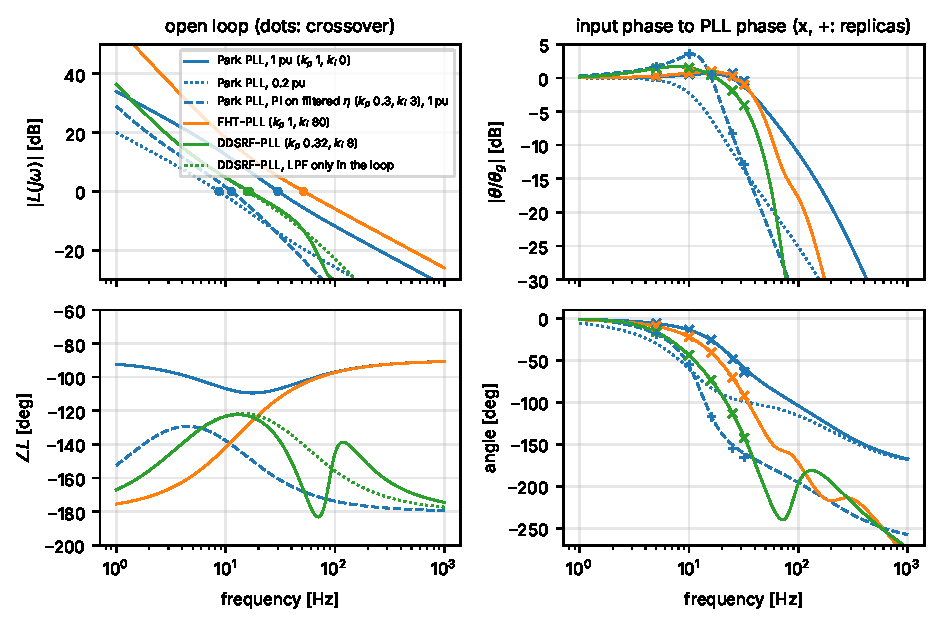
\includegraphics[width=\textwidth]{figures/pll_loops.pdf}
	\caption{Left: open loops $L(j\omega)$ (dots: crossover). Right: input phase to output phase $H$ of \eqref{eq:H}, with the front end outside the loop and the observer; crosses: the replicas of the model with a small phase modulation of the input; plus signs: the Park PLL with the PI on $\eta\ped{f}$.}
	\label{fig:loops}
\end{figure}

The replicas were run with a phase modulation of \num{2e-3} rad on a \SI{50}{\hertz} input, and the response read by a least-squares fit over \SI{1}{\second} (Table~\ref{tab:check}). The models of the FHT-PLL and of the DDSRF-PLL hold within \num{1}~\% up to \SI{200}{\radian\per\second}; with $F$ in place of $D\ped{eff}$ the DDSRF model would be \num{20}~\% off at \SI{200}{\radian\per\second}. The Park PLL is a single-phase loop in the strict sense: its detector reads the raw $u$, and the terms at $2\omega_0$ dropped in \eqref{eq:Kpd} mix a modulation at $W$ with its mirror $2\omega_0 - W$ (the loop is linear time-periodic \cite{golestan2017}). The averaged model holds within \num{1}~\% up to \SI{63}{\radian\per\second}, \num{3}~\% at \SI{100}{\radian\per\second} and \num{10}~\% at \SI{200}{\radian\per\second}; with the PI on $\eta\ped{f}$ it holds within \num{1.5}~\% up to \SI{63}{\radian\per\second}.

\begin{table}[H]
	\centering
	\caption{Input phase to output phase, replica against model: $|H|$ / angle at the modulation frequency $W$.}
	\label{tab:check}
	\footnotesize
	\setlength{\tabcolsep}{4pt}
	\begin{tabular}{@{} l l c c c c c @{}}
		\toprule
		 & & \multicolumn{5}{c@{}}{$W$ [rad/s]} \\
		loop & & 31.4 & 62.8 & 100 & 157 & 200 \\
		\midrule
		Park PLL & replica & 1.017 / \ang{-6.0} & 1.061 / \ang{-13.4} & 1.113 / \ang{-25.6} & 1.072 / \ang{-48.4} & 0.949 / \ang{-64.0} \\
		 & model & 1.016 / \ang{-6.1} & 1.053 / \ang{-13.9} & 1.077 / \ang{-26.1} & 0.987 / \ang{-46.7} & 0.858 / \ang{-59.2} \\
		\rowcolor{tableShade} FHT-PLL & replica & 1.032 / \ang{-9.4} & 1.090 / \ang{-22.1} & 1.117 / \ang{-40.6} & 1.028 / \ang{-70.6} & 0.893 / \ang{-92.0} \\
		\rowcolor{tableShade} & model & 1.032 / \ang{-9.4} & 1.090 / \ang{-22.1} & 1.117 / \ang{-40.7} & 1.024 / \ang{-70.7} & 0.887 / \ang{-92.0} \\
		DDSRF-PLL & replica & 1.178 / \ang{-16.2} & 1.190 / \ang{-44.1} & 1.051 / \ang{-73.7} & 0.804 / \ang{-113.6} & 0.624 / \ang{-142.5} \\
		 & model & 1.178 / \ang{-16.2} & 1.189 / \ang{-44.1} & 1.047 / \ang{-73.7} & 0.796 / \ang{-113.1} & 0.618 / \ang{-140.9} \\
		\rowcolor{tableShade} Park PLL on $\eta\ped{f}$ & replica & 1.212 / \ang{-18.5} & 1.505 / \ang{-55.5} & 1.062 / \ang{-117.4} & 0.387 / \ang{-154.5} & 0.228 / \ang{-165.6} \\
		\rowcolor{tableShade} & model & 1.214 / \ang{-18.7} & 1.483 / \ang{-56.5} & 1.004 / \ang{-116.3} & 0.371 / \ang{-150.8} & 0.219 / \ang{-160.7} \\
		\bottomrule
	\end{tabular}
\end{table}

The large-signal check is the \ang{+30} jump of case 2 (Figure~\ref{fig:jump}). The DDSRF-PLL follows its model within \ang{0.99}. The Park PLL differs by up to \ang{6.2}, a ripple at \SI{100}{\hertz} during the transient, while the generator is out of quadrature, that the averaged model leaves out: averaged over \SI{10}{\milli\second} the difference is \ang{0.71}. The FHT-PLL differs by \ang{4.1} (\ang{1.7} averaged): a \ang{30} error is beyond the linear range of the detector (the sine is \num{4.5}~\% short) and the normalization acts during the transient of the trackers. Overshoot in the simulation and in the model: \ang{4.67} and \ang{2.71} (Park), \ang{5.82} and \ang{4.31} (FHT-PLL), \ang{5.89} and \ang{5.54} (DDSRF-PLL).

\begin{figure}[H]
	\centering
	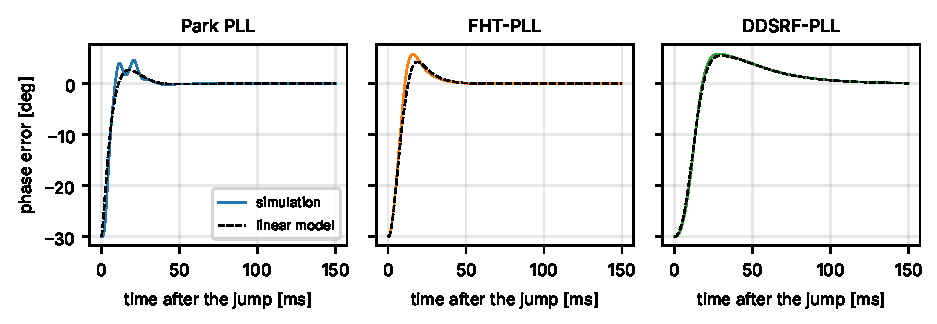
\includegraphics[width=\textwidth]{figures/jump_validation.pdf}
	\caption{Phase jump of \ang{+30} (case 2): phase error of the simulation and step response of the linear model \eqref{eq:H}.}
	\label{fig:jump}
\end{figure}

\subsection{Ripple from disturbances}
\label{sec:ripple}

With the complex gain of the front end (Section~\ref{sec:cgain}) each disturbance of the input becomes a set of components $c_k e^{jW_k t}$ of the frame vector, relative to the fundamental, and the steady-state ripple of the angle is
\begin{equation}
	\tilde\theta(t) = \sum_k \operatorname{Im}\big\{c_k\, T\ped{d}(jW_k)\, e^{jW_k t}\big\},
	\label{eq:ripple}
\end{equation}
with the disturbance transfer function $T\ped{d} = T$ for the FHT-PLL (the components enter the normalized detector as an angle), $T\ped{d} = O\,T/K\ped{pd}$ for the Park PLL (they enter after the detector of \eqref{eq:Kpd}) and $T\ped{d} = \omega_0 (k\ped{p}s + k\ped{i})\,D\ped{dd}(s)/\big(s^2 (1 + L)\big)$ for the DDSRF-PLL (each component goes through the network at its own frequency, with the complex coefficients of \eqref{eq:Ddd}). Table~\ref{tab:ripple} compares the prediction with the simulation. It holds within a few percent, except for the Park PLL on the DC offset: the DC term lands at $W = \omega_0$, which is its own mirror ($2\omega_0 - \omega_0 = \omega_0$), where the averaged detector cannot hold.

\begin{table}[H]
	\centering
	\caption{Steady-state ripple of the phase error (peak to peak): prediction \eqref{eq:ripple} and simulation.}
	\label{tab:ripple}
	\footnotesize
	\rowcolors{3}{tableShade}{white}
	\begin{tabular}{@{} l c c c c c c @{}}
		\toprule
		case & \multicolumn{2}{c}{Park PLL} & \multicolumn{2}{c}{FHT-PLL} & \multicolumn{2}{c@{}}{DDSRF-PLL} \\
		 & predicted & simulated & predicted & simulated & predicted & simulated \\
		\midrule
		1: 4th and 5th harmonic \SI{10}{\percent} & \ang{3.58} & \ang{3.39} & \ang{2.57} & \ang{2.59} & \ang{0.37} & \ang{0.39} \\
		4: DC offset \num{0.02} pu & \ang{2.73} & \ang{3.37} & \ang{2.06} & \ang{2.09} & \ang{1.39} & \ang{1.46} \\
		5: 3rd, 5th, 7th (EN 50160) & \ang{1.79} & \ang{1.78} & \ang{1.87} & \ang{1.93} & \ang{0.31} & \ang{0.31} \\
		\bottomrule
	\end{tabular}
	\rowcolors{1}{white}{white}
\end{table}

% =============================================================
\section{Results of the test cases}
\label{sec:results}

Table~\ref{tab:results} and Figure~\ref{fig:cases} give the six cases as simulated by the model (the logs; the replicas give the same numbers).

\begin{table}[H]
	\centering
	\caption{Test cases, PLLs as built (logs of the model): lock time, offset before the event, peak and settling time after it, final error and ripple (Section~\ref{sec:bench}). A dash: no event (case 5) or no settling within \ang{1} (the ripple is larger).}
	\label{tab:results}
	\footnotesize
	\rowcolors{2}{tableShade}{white}
	\begin{tabular}{@{} c l c c c c c c @{}}
		\toprule
		case & PLL & lock [ms] & offset & peak & settling [ms] & final error & ripple pp \\
		\midrule
		1 & Park PLL & 44 & \ang{0.00} & \ang{17.2} & -- & \ang{0.00} & \ang{3.39} \\
		 & FHT-PLL & 36 & \ang{1.49} & \ang{21.6} & -- & \ang{1.48} & \ang{2.59} \\
		 & DDSRF-PLL & 94 & \ang{0.85} & \ang{18.9} & 278 & \ang{0.78} & \ang{0.39} \\
		2 & Park PLL & 23 & \ang{0.00} & \ang{30.0} & 26 & \ang{0.00} & \ang{0.00} \\
		 & FHT-PLL & 25 & \ang{1.49} & \ang{30.0} & 33 & \ang{1.49} & \ang{0.01} \\
		 & DDSRF-PLL & 180 & \ang{0.72} & \ang{30.0} & 89 & \ang{0.74} & \ang{0.00} \\
		3 & Park PLL & 23 & \ang{0.00} & \ang{1.9} & 1 & \ang{1.15} & \ang{0.00} \\
		 & FHT-PLL & 25 & \ang{1.49} & \ang{2.5} & 2 & \ang{3.22} & \ang{0.03} \\
		 & DDSRF-PLL & 180 & \ang{0.72} & \ang{3.9} & 59 & \ang{1.61} & \ang{0.00} \\
		4 & Park PLL & 23 & \ang{0.00} & \ang{1.8} & -- & \ang{-0.03} & \ang{3.37} \\
		 & FHT-PLL & 25 & \ang{1.49} & \ang{1.2} & -- & \ang{1.49} & \ang{2.09} \\
		 & DDSRF-PLL & 180 & \ang{0.72} & \ang{1.1} & 18 & \ang{0.70} & \ang{1.46} \\
		5 & Park PLL & 22 & \ang{0.01} & -- & -- & \ang{0.01} & \ang{1.78} \\
		 & FHT-PLL & 25 & \ang{1.49} & -- & -- & \ang{1.49} & \ang{1.93} \\
		 & DDSRF-PLL & 140 & \ang{0.77} & -- & -- & \ang{0.77} & \ang{0.31} \\
		6 & Park PLL & 23 & \ang{0.00} & \ang{15.2} & 284 & \ang{0.00} & \ang{0.00} \\
		 & FHT-PLL & 25 & \ang{1.49} & \ang{20.5} & 275 & \ang{1.49} & \ang{0.01} \\
		 & DDSRF-PLL & 180 & \ang{-4.02}$^{*}$ & \ang{14.4}$^{*}$ & 278 & \ang{0.74} & \ang{0.00} \\
		\bottomrule
	\end{tabular}
	\rowcolors{1}{white}{white}
	\par\smallskip{\footnotesize $^{*}$ not settled before the sag at \SI{0.25}{\second} (\ang{18} peak to peak in the \SI{0.1}{\second} before it): the peak is not comparable; Section~\ref{sec:sag}.}
\end{table}

\begin{figure}[H]
	\centering
	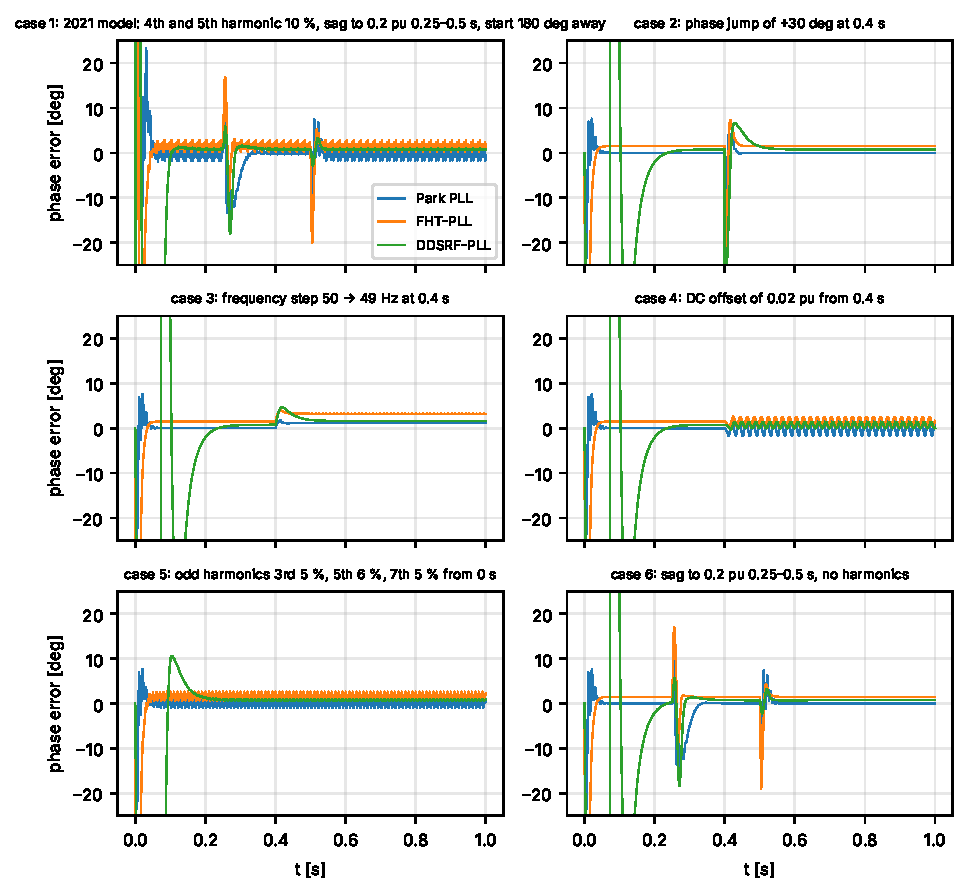
\includegraphics[width=\textwidth]{figures/cases_as_built.pdf}
	\caption{Phase error $e_\theta$ of the three PLLs as built on the six test cases (logs of the model). The axis is clipped at $\pm\ang{25}$: the start of case 1 from \ang{180} and the start of the DDSRF-PLL go beyond.}
	\label{fig:cases}
\end{figure}

\paragraph{Offsets.} The Park PLL has no offset: its generator is exact at the frequency of the PLL. The FHT-PLL locks \ang{1.49} ahead, the DDSRF-PLL \ang{0.72} to \ang{0.85} ahead (the angle of $G\ped{A}$ and of $G\ped{fht}$ at \SI{50}{\hertz}, Table~\ref{tab:qsg}).

\paragraph{Lock.} From \ang{180} away (case 1) the Park PLL locks in \SI{44}{\milli\second}, the FHT-PLL in \SI{36}{\milli\second}, the DDSRF-PLL in \SI{94}{\milli\second}. In the other cases the input starts in phase with the PLLs and the DDSRF-PLL takes the longest, \SI{180}{\milli\second}: its frequency integrator starts at the clamp, \num{0.5} pu, and the angle has to fall behind before the integrator can climb (Section~\ref{sec:critddsrf}).

\paragraph{Phase jump (case 2).} Settling within \ang{1} in \SI{26}{\milli\second} (Park), \SI{33}{\milli\second} (FHT-PLL) and \SI{89}{\milli\second} (DDSRF-PLL), as the crossovers of Table~\ref{tab:loops} say.

\paragraph{Frequency step to \SI{49}{\hertz} (case 3).} Final errors \ang{1.15}, \ang{3.22} and \ang{1.61}, with three different causes. The Park PLL has an adaptive generator but a type-1 loop: \ang{1.146} per hertz. The FHT-PLL and the DDSRF-PLL integrate the frequency, but their trackers stay tuned at \SI{50}{\hertz}: the angle of $G\ped{A}$ and of $G\ped{fht}$ at \SI{49}{\hertz}.

\paragraph{DC offset and harmonics (cases 4, 5, 1).} A DC offset of \num{0.02} pu gives a \SI{50}{\hertz} ripple of \ang{3.37} (Park), \ang{2.09} (FHT-PLL), \ang{1.46} (DDSRF-PLL); the EN 50160 harmonics \ang{1.78}, \ang{1.93} and \ang{0.31}; the 4th and 5th harmonic of case 1 \ang{3.39}, \ang{2.59} and \ang{0.39}. The Park PLL pays for its detector on the raw input; the FHT-PLL, whose stage A is the most selective, for its fast loop ($|T(j2\omega_0)| = 0.475$); the DDSRF-PLL is the best on harmonics because its network and its slow loop filter what the single tracker lets through. Section~\ref{sec:ripple} predicts all these numbers from the front ends and the loops.

\subsection{Sags}
\label{sec:sag}

The sag to \num{0.2} pu (case 6) gives the largest errors of the tests: \ang{15.2} at the start and \ang{15.1} at the end for the Park PLL, \ang{15.5} and \ang{20.5} for the FHT-PLL, \ang{19.2} and \ang{3.0} for the DDSRF-PLL. They are not a fault of the loops. A step of the amplitude moves the angle of the vector that a generator builds (Figure~\ref{fig:sag}, top): in the first \SI{20}{\milli\second} the angle of $u + j\beta$ of the Park generator deviates by up to \ang{45.3} at the start of the sag and \ang{31.5} at its end, the angle of $\alpha + j\beta$ of the tracker by \ang{47.1} and \ang{27.8}, while the input keeps its phase. Any generator with a settling time of some milliseconds turns an amplitude step into a phase transient of this size, and the loop follows part of it. The DDSRF-PLL is the best at the end of the sag and not at its start, partly because its detector divides the filtered $\operatorname{Im} y\ped{p}$ by the instantaneous magnitude of the tracker output.

\begin{figure}[H]
	\centering
	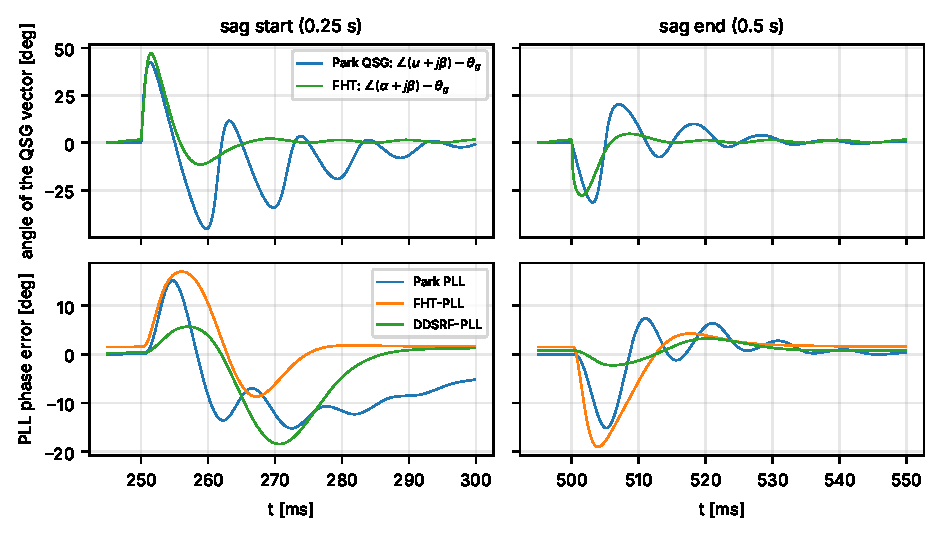
\includegraphics[width=\textwidth]{figures/sag_edges.pdf}
	\caption{Sag to \num{0.2} pu (case 6). Top: angle of the vector built by the generators minus $\theta\ped{g}$ (Park: $u + j\beta$; FHT: $\alpha + j\beta$ of the first tracker). Bottom: phase error of the three PLLs. Left: start of the sag at \SI{0.25}{\second}; right: end at \SI{0.5}{\second}.}
	\label{fig:sag}
\end{figure}

% =============================================================
\section{Criticalities and changes}
\label{sec:crit}

The changes below were tested on the replicas with the six cases (Table~\ref{tab:var}, Figure~\ref{fig:var}) and, for the start, with the input at six initial phases (Table~\ref{tab:lock}). Three of them are recommended; the others are options with a price.

\begin{table}[H]
	\centering
	\caption{Changes tested on the replicas: lock time, ripple and peak in case 1, settling in case 2, final error and peak in case 3, ripple in cases 4 and 5, peak in case 6. First row of each PLL: as built.}
	\label{tab:var}
	\footnotesize
	\setlength{\tabcolsep}{3.5pt}
	\rowcolors{3}{tableShade}{white}
	\begin{tabular}{@{} l l c c c c c c c c c @{}}
		\toprule
		 & & \multicolumn{3}{c}{case 1} & case 2 & \multicolumn{2}{c}{case 3} & case 4 & case 5 & case 6 \\
		PLL & variant & lock [ms] & pp & peak & settl.\ [ms] & final & peak & pp & pp & peak \\
		\midrule
		Park & as built ($k\ped{i}$ 0) & 44 & 3.39 & 17.2 & 26 & 1.15 & 1.85 & 3.37 & 1.78 & 15.2 \\
		Park & $k\ped{i}$ 20 & 57 & 3.41 & 18.1 & 37 & 0.00 & 1.63 & 3.59 & 1.79 & 17.2 \\
		Park & $k\ped{i}$ 20, normalized $\eta$ & 159 & 3.43 & 38.7 & 36 & 0.00 & 1.63 & 3.59 & 1.80 & 39.7 \\
		Park & $k\ped{i}$ 20, DC estimate $0.02\,\omega_0$ & 57 & 3.43 & 20.1 & 62 & 0.00 & 1.65 & 0.16 & 1.79 & 20.2 \\
		Park & PI on $\eta\ped{f}$, $k\ped{p}$ 0.3, $k\ped{i}$ 3 & 205 & 0.14 & 6.9 & 141 & 0.02 & 5.09 & 0.44 & 0.12 & 3.0 \\
		FHT-PLL & as built & 36 & 2.59 & 21.6 & 33 & 3.22 & 2.49 & 2.09 & 1.93 & 20.5 \\
		FHT-PLL & undamped trackers & 41 & 2.62 & 22.1 & 33 & 1.74 & 2.49 & 2.04 & 1.97 & 21.0 \\
		FHT-PLL & undamped, DC state $-0.1\,\omega_0$ & 42 & 2.57 & 25.4 & 45 & 1.98 & 2.73 & 0.00 & 1.97 & 24.5 \\
		FHT-PLL & SOGI poles $k = 1$ & 34 & 0.14 & 11.5 & 45 & 4.67 & 5.00 & 0.96 & 0.15 & 11.5 \\
		DDSRF & as built & 94 & 0.39 & 18.9 & 89 & 1.61 & 3.95 & 1.46 & 0.31 & 14.4 \\
		DDSRF & start 1 pu, undamped tracker & 125 & 0.40 & 19.2 & 89 & 0.87 & 3.94 & 1.45 & 0.32 & 18.9 \\
		DDSRF & start 1 pu, DC state $-0.5\,\omega_0$ & 114 & 0.45 & 15.3 & 90 & 1.34 & 4.32 & 0.00 & 0.37 & 15.0 \\
		DDSRF & start 1 pu, SOGI poles $k = 1$ & 132 & 0.09 & 17.7 & 93 & 2.34 & 5.17 & 1.00 & 0.09 & 18.4 \\
		\bottomrule
	\end{tabular}
	\rowcolors{1}{white}{white}
	\par\smallskip{\footnotesize Angles in degrees. The DC state is a third state of the tracker, $u = x_1 + x_3$ with $\dot x_3 = l_3(u - x_1 - x_3)$, pole as given; ``SOGI poles $k = 1$'': undamped tracker with the poles $\omega_0(-0.5 \pm 0.866j)$ of a SOGI with $k = 1$.}
\end{table}

\begin{figure}[H]
	\centering
	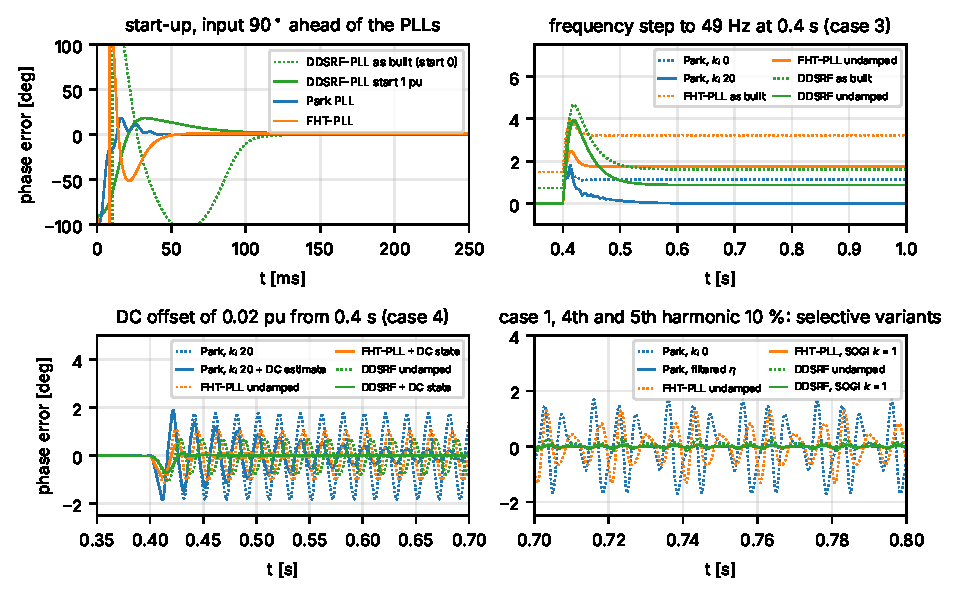
\includegraphics[width=\textwidth]{figures/variants.pdf}
	\caption{Changes on the replicas. Top left: start with the input \ang{90} ahead (no event): DDSRF-PLL with the frequency integrator as built (clamped at \num{0.5} pu) and started at \num{1} pu, Park PLL and FHT-PLL as built. Top right: frequency step to \SI{49}{\hertz} (case 3). Bottom left: DC offset (case 4), error minus its value before the offset. Bottom right: case 1 after the sag, with the 4th and 5th harmonic: the selective variants against the PLLs as built.}
	\label{fig:var}
\end{figure}

\subsection{Park PLL}
\label{sec:critpark}

\begin{enumerate}
	\item \textbf{Type-1 loop (recommended: $k\ped{i} = 20$).} With $k\ped{i} = 0$ a frequency step leaves \ang{1.15} per hertz at \num{1} pu and \ang{5.7} per hertz at \num{0.2} pu. With $k\ped{i} = 20$ the error goes to zero; the margin stays \ang{66.8} at \num{1} pu and \ang{54.7} at \num{0.2} pu, the jump settles in \SI{37}{\milli\second} instead of \SI{26}{\milli\second}, the lock from \ang{180} takes \SI{57}{\milli\second} instead of \SI{44}{\milli\second}, nothing else changes. A parameter of the init, \code{param.afe.pll.park.ki}.
	\item \textbf{Detector on the raw input.} Harmonics and DC bypass the generator ($|G\ped{park}| \approx 0.5$, Table~\ref{tab:qsg}): \ang{3.4} of ripple in case 1, \ang{3.4} with \num{2}~\% of DC, \ang{1.8} with the EN 50160 harmonics, \ang{15} at the sag edges. The block already computes the detector of the SOGI-PLL, $\eta\ped{f}$; feeding the PI with it is one line in the model and brings the ripple to \ang{0.14}, \ang{0.44} and \ang{0.12} and the sag peak to \ang{3.0}. The price is speed: the generator pole $\omega\ped{f}/2 = \SI{78.5}{\radian\per\second}$ enters the loop \eqref{eq:Kpd}, the PI must be slowed to $k\ped{p} = 0.3$, $k\ped{i} = 3$ (crossover \SI{71}{\radian\per\second}, margin \ang{40} at \num{1} pu and \ang{49} at \num{0.2} pu, Table~\ref{tab:loops}), the jump settles in \SI{141}{\milli\second}, the frequency step peaks at \ang{5.1} and the lock from \ang{180} takes \SI{205}{\milli\second}. An option for an application where the harmonics matter more than the speed; a larger gain $k$ of the generator (a shorter $\tau$) moves the pole up and gives back part of the speed for part of the selectivity.
	\item \textbf{No normalization.} The loop gain follows the amplitude: the crossover falls from \SI{189}{} to \SI{55}{\radian\per\second} at \num{0.2} pu. Dividing $\eta$ by the magnitude of the filtered pair, as the other two loops do, keeps the dynamics in the sag but doubles the errors at its edges (\ang{38.7} and \ang{39.7}) and slows the lock (\SI{159}{\milli\second}): the magnitude estimate is as slow as the generator. Not recommended with this generator.
	\item \textbf{DC offset.} A DC estimate subtracted from the input, $d[k+1] = d[k] + t\ped{s}\, g\,(u[k] - d[k] - \hat\alpha[k])$ with $g = 0.02\,\omega_0$ (the third integrator of a SOGI with DC rejection), removes the \SI{50}{\hertz} ripple (\ang{0.16} instead of \ang{3.59}) but settles the jump in \SI{62}{\milli\second} and adds \ang{2} to \ang{3} at the sag edges. An option where the measurement has an offset.
\end{enumerate}

\subsection{FHT-PLL}
\label{sec:critfht}

\begin{enumerate}
	\item \textbf{Offset at \SI{50}{\hertz} (recommended: undamped trackers).} The damped, forward Euler model of the class gives \ang{1.49} at \SI{50}{\hertz} and \ang{3.22} at \SI{49}{\hertz} (Section~\ref{sec:fht}). The undamped oscillator with the exact discretization (\code{param.afe.pll.fht\_undamped = true}) removes the offset at \SI{50}{\hertz} and halves the error at \SI{49}{\hertz} (\ang{1.74}); nothing else changes. The option is in the init of the model; the change belongs in the class \code{ctrl\_afe\_setup} of the library (\code{first\_harmonic\_tracker}), which the AFE models share (in \code{frt\_dqpll} the C code of the tracker adds its own lead \cite{note_3ph}).
	\item \textbf{Fixed tuning.} The trackers do not follow the frequency: \ang{0.87} per tracker at \SI{49}{\hertz} even undamped, and stage A doubles it. Feeding the frequency of the loop to the trackers is the cure; a first attempt in the replicas, with the unfiltered frequency of stage B, lost the lock. It needs its own design: open point.
	\item \textbf{Wide trackers.} The poles $-\omega_0$, $-4\omega_0$ make the tracker fast and let harmonics and DC through: the ripple of the FHT-PLL is close to that of the Park PLL. Narrower trackers, with the poles of a SOGI with $k = 1$, cut the harmonic ripple by \num{18} (\ang{0.14} in case 1, \ang{0.15} in case 5) and halve the sag peaks, but the error at \SI{49}{\hertz} grows to \ang{4.67}: a narrow filter at a fixed frequency. Only together with item 2. A DC state in the tracker (third state, pole $-0.1\,\omega_0$) removes the DC ripple (\ang{0.00} instead of \ang{2.04}) for \SI{12}{\milli\second} more of settling and \ang{3} to \ang{4} more at the sag edges.
\end{enumerate}

\subsection{DDSRF-PLL}
\label{sec:critddsrf}

\begin{enumerate}
	\item \textbf{Start (recommended: frequency integrator at \num{1} pu).} The integrator starts at zero and the clamp holds it at \num{0.5} pu: the loop has to catch up half the frequency, and the lock takes \SI{94}{} to \SI{180}{\milli\second} depending on the initial phase, the longest when the input starts in phase with the PLL (Table~\ref{tab:lock}, Figure~\ref{fig:var}). Started at \num{1} pu (initial condition of the integrator, inside the clamp) the lock takes \SI{0}{} to \SI{135}{\milli\second}. The block is the one of \code{frt\_dqpll}: the same change applies there.
	\item \textbf{Offset (recommended: undamped tracker).} \ang{0.74} at \SI{50}{\hertz} and \ang{1.61} at \SI{49}{\hertz} from the tracker; undamped: \ang{0} and \ang{0.87} (item 1 of the FHT-PLL).
	\item \textbf{Slow loop.} The network in the loop limits the crossover to about \SI{100}{\radian\per\second}: the jump settles in \SI{89}{\milli\second} against \SI{26}{} to \SI{33}{\milli\second} of the other two. It is the price of the exact cancellation of the image and of the lowest harmonic ripple; in a single-phase grid the ``negative sequence'' is only the image of the tracker (\num{0.014} at \SI{50}{\hertz}, zero with the undamped tracker).
	\item \textbf{DC and selectivity.} As for the FHT-PLL, a DC state removes the DC ripple and SOGI poles cut the harmonic ripple, with the same costs (Table~\ref{tab:var}).
\end{enumerate}

\begin{table}[H]
	\centering
	\caption{Lock time [ms] against the initial phase of the input (no event, \SI{50}{\hertz}, replicas): DDSRF-PLL as built and with the frequency integrator started at \num{1} pu, Park PLL and FHT-PLL as built.}
	\label{tab:lock}
	\footnotesize
	\rowcolors{2}{tableShade}{white}
	\begin{tabular}{@{} c c c c c @{}}
		\toprule
		initial phase & DDSRF-PLL as built & DDSRF-PLL start \num{1} pu & Park PLL & FHT-PLL \\
		\midrule
		\ang{0} & 180 & 0 & 23 & 25 \\
		\ang{45} & 116 & 62 & 30 & 21 \\
		\ang{90} & 105 & 83 & 30 & 42 \\
		\ang{135} & 99 & 98 & 36 & 39 \\
		\ang{170} & 95 & 116 & 42 & 37 \\
		\ang{180} & 94 & 135 & 44 & 37 \\
		\bottomrule
	\end{tabular}
	\rowcolors{1}{white}{white}
\end{table}

\subsection{Common points}
\label{sec:critcommon}

\begin{itemize}[nosep]
	\item \textbf{Sag edges.} The errors of \ang{15} to \ang{20} at the edges of a sag (Section~\ref{sec:sag}) come from the generators and remain with every change of the table but the selective ones. Holding the integrator and the frequency of the loop for a few milliseconds after an amplitude step, detected on the magnitude of the generator output, is the usual measure; it was not tested here: open point.
	\item \textbf{Ideal signal.} The model feeds the PLLs with an exact, noiseless sample of the voltage. A real control adds the delay of the acquisition (one control period is \ang{2.25} at \SI{50}{\hertz}) and its quantization, the same for the three loops.
	\item \textbf{Two outputs.} The Park PLL gives the observer angle $\hat\theta$, the other two the loop angle $\theta$; the three give the observer frequency, about \SI{4}{\milli\second} behind the loop.
\end{itemize}

% =============================================================
\section{Summary}
\label{sec:summary}

Table~\ref{tab:summary} puts the three loops side by side. For a single-phase grid the Park PLL with $k\ped{i} = 20$ is the simplest good choice when speed matters and the harmonics are moderate; with the PI on $\eta\ped{f}$ it becomes the SOGI-PLL, with a ripple twenty times lower and a five times slower response. The FHT-PLL and the DDSRF-PLL are the loops of the three-phase AFE control adapted to one phase: with the undamped tracker and, for the DDSRF-PLL, the integrator started at \num{1} pu, the FHT-PLL is as fast as the Park PLL with a fixed tuning, and the DDSRF-PLL has the lowest ripple of the three loops as built at the price of the slowest response.

\begin{table}[H]
	\centering
	\caption{The three PLLs at a glance (Tables~\ref{tab:results} and \ref{tab:var}).}
	\label{tab:summary}
	\footnotesize
	\rowcolors{2}{tableShade}{white}
	\begin{tabularx}{\textwidth}{@{} >{\raggedright\arraybackslash}p{0.2\textwidth} X X X @{}}
		\toprule
		& Park PLL & FHT-PLL & DDSRF-PLL \\
		\midrule
		generator & SOGI $k = 0.5$ by Park transforms, adaptive, inside the loop; detector on the raw input & three trackers, fixed at \SI{50}{\hertz}, outside the loop & one tracker outside the loop, decoupling network inside \\
		offset at \SI{50}{\hertz} & none & \ang{1.49} & \ang{0.74} \\
		frequency step to \SI{49}{\hertz} & \ang{1.15} (type 1) & \ang{3.22} (fixed trackers) & \ang{1.61} (fixed tracker) \\
		jump \ang{30}, settling & \SI{26}{\milli\second} & \SI{33}{\milli\second} & \SI{89}{\milli\second} \\
		harmonics, EN 50160 / case 1 & \ang{1.78} / \ang{3.39} & \ang{1.93} / \ang{2.59} & \ang{0.31} / \ang{0.39} \\
		DC offset \num{0.02} pu & \ang{3.37} & \ang{2.09} & \ang{1.46} \\
		sag to \num{0.2} pu, start / end & \ang{15.2} / \ang{15.1} & \ang{15.5} / \ang{20.5} & \ang{19.2} / \ang{3.0} \\
		lock (any initial phase) & \SI{23}{} to \SI{44}{\milli\second} & \SI{21}{} to \SI{42}{\milli\second} & \SI{94}{} to \SI{180}{\milli\second} \\
		what to change & $k\ped{i} = 20$; option: PI on $\eta\ped{f}$ & undamped trackers; open: adaptive tuning & integrator started at \num{1} pu, undamped tracker \\
		\bottomrule
	\end{tabularx}
	\rowcolors{1}{white}{white}
\end{table}

% =============================================================
\section{Files and how to reproduce}
\label{sec:files}

\begin{itemize}[nosep]
	\item \code{foundations\us of\us power\us electronics/\allowbreak single\us phase\us dqPLLs\us analysis} of \cite{model_repo}: the model \code{single\_phase\_pll\_analysis.slx}; its init \code{init\_model.m} (plain-text live script, struct \code{param}, design check \code{pll\_design} with the models of Section~\ref{sec:models}); \code{run\_test\_cases.m} (simulates the six cases, prints the metrics, saves the logs); \code{plotting\_results\_plls.m} (input, phase errors and frequencies of a run or of a saved file); the functions of \code{private/} (test signals, timing, metrics, design check, checks of the model); the README with the parameters and the names of the old init.
	\item This folder: \code{py/sp\_pll\_models.py} (the replicas of the three blocks and their variants, the test signal, the metrics) and \code{py/make\_figures.py} (every figure and number of the note, written to \code{figures/\allowbreak single\us phase\us pll\us numbers.txt}).
	\item To reproduce: in MATLAB, in the model folder, \code{init\_model} and then \code{run\us test\us cases(1:6, \allowbreak 'sim\us results\us cases.mat')}; in Python, in the folder \code{py}, \code{python3 make\us figures.py \allowbreak path/\allowbreak to/\allowbreak sim\us results\us cases.mat} (about \SI{30}{\second}). Without the file the script runs the test cases on the replicas, with the same numbers.
	\item The library \cite{library_repo}: \code{setup\_files/objs/ctrl\_afe\_setup.m} (trackers \code{fht\_grid}, observer \code{di\_obs}, loop gains), \code{masked\_models/filters/discrete\_time\_low\_pass\_filter.slx}.
\end{itemize}

% =============================================================
\begin{thebibliography}{9}
	\raggedright
	\bibitem{model_repo} pwr-control, \emph{modelization-and-control}, repository, folder \code{foundations\us of\us power\us electronics/\allowbreak single\us phase\us dqPLLs\us analysis} (model \code{single\_phase\_pll\_analysis.slx}, README with the design check of November 2026). \url{https://github.com/pwr-control/modelization-and-control}
	\bibitem{library_repo} pwr-control, \emph{library}, repository: setup classes (\code{ctrl\_afe\_setup}), masked blocks (\code{discrete\_time\_low\_pass\_filter}), stage B of the PLLs. \url{https://github.com/pwr-control/library}
	\bibitem{note_3ph} D. Bagnara, \emph{Three-phase grid PLLs under grid faults: dq-PLL, DDSRF-PLL and FHT-PLL of the model frt\_dqpll}, pwr-control technical note, rev.~00, November 2026, \code{repos\_doc/three\_phase\_plls\_comparison} of \emph{repositories-documentation}.
	\bibitem{ciobotaru2006} M. Ciobotaru, R. Teodorescu and F. Blaabjerg, ``A new single-phase PLL structure based on second order generalized integrator,'' \emph{37th IEEE Power Electronics Specialists Conference (PESC)}, 2006.
	\bibitem{teodorescu2011} R. Teodorescu, M. Liserre and P. Rodr\'iguez, \emph{Grid Converters for Photovoltaic and Wind Power Systems}, Wiley, 2011, chapter 4 (grid synchronization in single-phase power converters).
	\bibitem{rodriguez2007} P. Rodr\'iguez, J. Pou, J. Bergas, J. I. Candela, R. P. Burgos and D. Boroyevich, ``Decoupled double synchronous reference frame PLL for power converters control,'' \emph{IEEE Transactions on Power Electronics}, vol.~22, no.~2, pp.~584--592, 2007.
	\bibitem{golestan2017} S. Golestan, J. M. Guerrero and J. C. Vasquez, ``Single-phase PLLs: a review of recent advances,'' \emph{IEEE Transactions on Power Electronics}, vol.~32, no.~12, pp.~9013--9030, 2017.
	\bibitem{en50160} EN 50160:2010, \emph{Voltage characteristics of electricity supplied by public electricity networks}, CENELEC, 2010.
\end{thebibliography}

\end{onehalfspace}
\end{document}
